\documentclass[11pt,a4paper]{report}

\usepackage[utf8]{inputenc}
\usepackage[T1]{fontenc}
\usepackage[english]{babel}
\usepackage{graphicx}
\usepackage{booktabs}
\usepackage{amsmath,amssymb}
\usepackage{listings}
\usepackage{xcolor}
\usepackage{caption}
\usepackage{subcaption}
% The generated table captions run to several hundred words. The caption
% package's single-line check boxes the whole caption on one line to measure
% it, and for those captions the box exceeds TeX's maximum dimension. The
% check is pointless for captions that long, so it is disabled for tables.
\captionsetup[table]{singlelinecheck=false,font=footnotesize}
\usepackage[hidelinks]{hyperref}
\usepackage[margin=2.0cm]{geometry}
% Centred chapter headings, at the report class's own vertical spacing so the
% page count is unaffected.
\usepackage{titlesec}
\titleformat{\chapter}[display]
  {\normalfont\huge\bfseries\centering}{\chaptertitlename\ \thechapter}{20pt}{\Huge}
\titlespacing*{\chapter}{0pt}{50pt}{40pt}
\usepackage{tikz}
\usetikzlibrary{arrows.meta,positioning,shapes.geometric}

\graphicspath{{figures/}{../results/figures/}}

\title{%
  \textbf{Agentic AI for Information Retrieval}\\[0.4em]
  \large A Multi-Agent System for Multi-Hop Retrieval with\\
  Self-Reflective Validation
}
\author{%
  Student ID: D03000104\\[0.6em]
  \small Universit\`a degli Studi di Napoli Federico II\\
  \small Information Retrieval, A.Y. 2024/2025\\
  \small Prof. Antonio Maria Rinaldi and Dr. Domenico Benfenati\\
  \small IKNOS-DIETI Lab
}
\date{\today}

% Chapters and sections only: subsections in the contents cost a page.
\setcounter{tocdepth}{1}

\begin{document}

\maketitle
\tableofcontents

\begin{abstract}
Most retrieval-augmented systems retrieve once and generate once, and that
structure cannot answer a question whose evidence is spread across documents,
because no single document is rankable as the answer. This report presents an
agentic alternative: four agents coordinated by an explicit state machine,
covering all five tasks of the assignment brief. A Planner decomposes a
question into a validated graph of dependent sub-queries, a Retrieval Agent
routes each to BM25, dense or hybrid search, a Knowledge Graph Navigator
recovers bridge entities from a graph induced from corpus text, and a Verifier
scores the answer against its own citations. The central contribution is one
backward edge: below its confidence threshold the Verifier returns a re-plan
directive to the Planner instead of an answer. Everything runs locally on one
consumer GPU with no paid API, and the edge is isolated by ablation rather
than asserted.

The result is reported as measured. On answer accuracy the agentic system does
not lead: exact match is 0.432 on HotpotQA and 0.224 on 2WikiMultihopQA against
0.504 and 0.264 for a self-ask baseline that decomposes but never verifies.
The backward edge does measurable work on one dataset and none on the other.
The largest effect in the ablation grid belongs to the component the brief
lists first, and its sign is negative: deleting the Planner improves F1 by
0.121 on 2WikiMultihopQA at a third of the model calls. What the agentic stack
earns its cost for is grounded, auditable answers, with 0.960 and 0.976 of
citations resolving to real sentences where no baseline's resolve at all.

A bounded improvement loop then tested five hypotheses against the one-node
configuration. One survived: letting the synthesiser reason, with a completion
budget large enough to hold it, takes exact match to 0.524 and 0.456, ties the
strongest baseline on HotpotQA and beats it by 0.192 on 2WikiMultihopQA. The
loop also established that seed pinning does not make this system
reproducible, because a caching inference server changes the arithmetic
between identical requests, and that finding bounds every comparison in this
report.
\end{abstract}

\chapter{Introduction to Agentic AI in Information Retrieval}
\label{ch:introduction}

\section{From Reactive Generation to Agency}

A generative language model is a function from a prompt to a completion. It
emits text and stops. It holds no goal that outlives the call, it cannot observe
what its output caused, and it has no way of concluding that what it produced
was not good enough. That describes a component, and it also describes most
systems currently called retrieval-augmented: embed a query, fetch a ranked
list, paste the list into a prompt, emit a completion. Retrieve once, generate
once. Nothing in that structure allows the behaviour to be anything but
reactive.

Agentic artificial intelligence names the class of systems built to remove that
limitation. An agentic system pursues a goal across several steps, chooses its
own actions, calls external instruments to carry them out, observes what came
back, and revises its behaviour in light of the
observation~\cite{zhang2024aiagent,wu2025agentic}. Four properties carry the
weight. \textbf{Autonomy}: the system, not the user, decides what happens next.
\textbf{Goal-directed planning}: the work is represented explicitly before it
is done, so the plan can be inspected, validated, repaired and discarded.
\textbf{Tool integration}: the model is not the source of facts but the
selector of instruments. \textbf{Adaptive reasoning}: the plan can be revised
after execution has begun, because an observation can invalidate it.

The fourth property is the difficult one and the one most often missing. A
system can be autonomous, planned and tool-using and still be a fixed pipeline
whose stages happen to be model calls. The industry touchstones the assignment
brief names, AutoGPT and Microsoft's Jarvis, are notable for attempting the
fourth property. The research literature shows the same direction. PaperQA
retrieves across scientific articles, judges what it found and synthesises from
the survivors~\cite{lala2023paperqa}. Agentic Reasoning adds tool-using
sub-agents and a mind-map agent~\cite{wu2025agentic}. CollEX explores
multimodal scientific collections~\cite{schneider2025collex}, agentic
contextual retrieval in telecommunications combines multi-source retrieval
with self-reflective validation~\cite{zhang2025toward}, and multi-agent
geospatial copilots decompose remote-sensing workflows across specialised
agents~\cite{lee2025multiagent}. What they share is the shape, and what they
leave open is the question this report exists to test: whether the feedback
edge, once actually implemented, earns the compute it consumes.

\section{The Limits of Static Ranking}

Classical information retrieval is the study of a scoring function. Given a
query and a corpus, rank the documents and return the top $k$. BM25 formalises
this for lexical matching~\cite{robertson2009probabilistic}, dense bi-encoders
replace term overlap with proximity in a learned space~\cite{xiao2023cpack},
reciprocal rank fusion combines rankings whose scores share no
scale~\cite{cormack2009reciprocal}, and BEIR measures how well any of it
transfers~\cite{thakur2021beir}. These are real and cumulative advances, and
every one of them improves the ordering of a single list produced from a
single query.

Consider a HotpotQA question~\cite{yang2018hotpotqa} that this report reuses
throughout:

\begin{quote}
\textit{When did the tour begin for the album Taylor Swift released on
October 22, 2012?}
\end{quote}

\noindent The passage \texttt{Red (Taylor Swift album)} says the album was
released on that date. The passage \texttt{The Red Tour} says the tour began on
March 13, 2013. Of the 66{,}581 passages in the processed HotpotQA corpus, none
contains both dates. That is not a statement about ranking quality. There is no
document for a ranker to place first, because no single document answers the
question. The bridge entity, the album title \textit{Red}, does not occur in
the question at all; it has to be derived before it can be searched for. A
lexical retriever cannot match a term that was never typed, and a dense
retriever embeds the whole question, so the sub-need ``identify the album'' is
diluted by the sub-need ``find its tour date'' rather than issued on its own.
This is the compositionality gap that Press et al.\ measure
directly~\cite{press2023selfask}, and it is what motivates interleaving
retrieval with reasoning rather than separating them~\cite{trivedi2023interleaving}.

Scale turns the difficulty into an impossibility. The two corpora hold
66{,}581 and 54{,}957 passages, so the number of ordered passage pairs is on
the order of $10^9$. The composition cannot be materialised in advance; it has
to be inferred from the question, which is a reasoning operation rather than a
ranking one. Two pressures compound it: the distractor setting fills each
candidate pool with passages chosen to look like the gold ones, and relevance
for the first hop is defined only relative to an intermediate goal the user
never stated.

\section{Problem Statement}

The problem is the design of a retrieval agent that, given a question and a
static corpus, does four things a ranker does not. It interprets an intent
whose surface form under-specifies the work. It decomposes that intent into
ordered sub-goals with explicit dependencies, so that one retrieval's result
can be substituted into the next query. It orchestrates the resulting workflow,
choosing an instrument for each sub-goal and traversing structure where the
corpus admits one. And it judges its own answer against the evidence it
actually retrieved before returning anything.

The fourth requirement is where a pipeline and an agent part company. The
system described here is, with one exception, a forward pipeline: plan,
execute, aggregate, synthesise. The exception is a single backward edge. A
Verifier scores each candidate answer against the evidence cited for it, and
when its confidence falls below a threshold it does not answer. It sends a
\texttt{ReplanDirective} back to the Planner carrying what could not be
established, which sub-queries returned nothing useful, and the text of every
sub-query already tried, which the next plan may not repeat. One edge is a
modest architectural change and a categorical behavioural one.

The system runs entirely on local hardware: \texttt{qwen3:8b} at Q4\_K\_M
quantisation through Ollama on a single RTX 5060 with 8~GB of VRAM, measured at
52 tokens per second warm, with no API key anywhere. At that throughput a
schema-constrained model call costs several seconds, so every call has to be
justified against a deterministic alternative. Tool selection is a decision
table over lexical features, entity linking is alias matching, graph traversal
is breadth-first search, and the confidence blend is arithmetic. A system that
cannot afford to think everywhere is forced to say where thinking pays, and, as
Chapter~\ref{ch:implementation} reports, the answer it arrived at was not the
one it was designed around.

\section{Objectives and Contributions}

The objective is a working agentic retrieval system covering all five tasks of
Table~1 of the assignment brief, whose central claim is tested rather than
asserted. The contributions are four.

\textbf{A four-agent architecture with full task coverage.} A Planner emits a
validated directed acyclic graph of sub-queries linked by placeholders. A
Retrieval Agent selects among BM25, dense and hybrid search under a conditional
reranking gate. A Knowledge Graph Navigator traverses an entity graph built from
corpus text alone. A Verifier performs self-reflective validation. An
orchestrator specified as an explicit state machine coordinates the four.

\textbf{The Verifier-to-Planner feedback loop, isolated by ablation.} A
configuration with the backward edge disabled and everything else held fixed
measures what the loop is worth, and the trace records which cycle produced the
selected answer.

\textbf{An evaluation protocol that prices agency.} Answer and retrieval quality
are reported beside model calls, tool calls, plan depth, re-plan rate and
latency, so no gain appears without its cost. Nine configurations run over two
multi-hop benchmarks, all eighteen cells on the same frozen 250 questions.

\textbf{A local, reproducible implementation, and an honest account of how
reproducible.} Every model runs on-device, prompts are versioned files whose
rendered hash is logged, and a test asserts that no module reaches the network.
Section~\ref{sec:reproducibility} reports the measured limit of that
reproducibility, which turned out to be a finding in its own right.

Table~\ref{tab:task-mapping} records where each task of the brief is
implemented and measured. One clause of the brief is deliberately not met: it
mentions orchestrating external APIs for real-time enrichment, and this system
exposes no external API at all, because a tool whose output changes between
runs makes the evaluation unrepeatable and the trace unfalsifiable. The
registry is written so that such a connector could be added as one more entry.

\begin{table}[htbp]
  \centering
  \small
  \caption{The five tasks of the brief's Table~1, the component implementing
  each, and where the report specifies and measures it. Four agents cover five
  tasks because query refinement and retrieval planning are one act performed
  twice: before any evidence exists, and again after the Verifier has said what
  is missing.}
  \label{tab:task-mapping}
  \begin{tabular}{p{4.0cm}p{4.6cm}p{5.6cm}}
    \toprule
    Task (brief, Table~1) & Agent or component & Specified in; measured in \\
    \midrule
    Autonomous query refinement &
      Planner: per-node rewrites; re-plan on a directive &
      \S\ref{sec:decomposition}, \S\ref{sec:verification};
      re-plan rate in Table~\ref{tab:agent-metrics-hotpotqa} \\
    Multi-step retrieval planning &
      Planner: validated sub-query DAG; orchestrator state machine &
      \S\ref{sec:decomposition}, \S\ref{sec:architecture};
      \S\ref{sec:ablations} \\
    Tool-augmented retrieval &
      Retrieval Agent: registry, routing table, reranking gate &
      \S\ref{sec:tools}; Table~\ref{tab:agent-metrics-hotpotqa} \\
    Knowledge graph traversal &
      KG Navigator: alias linking, bidirectional BFS &
      \S\ref{sec:kg-traversal}, \S\ref{sec:preprocessing};
      \S\ref{sec:ablations} \\
    Self-reflective validation and fact checking &
      Verifier: NLI entailment, citation grounding, feedback edge &
      \S\ref{sec:verification}; \S\ref{sec:ablations}, \S\ref{sec:errors} \\
    \bottomrule
  \end{tabular}
\end{table}

A fifth outcome was not designed but is reported because it is useful. During
development the 8B model produced correctly shaped decompositions in 8 of 8
cases with no format retries, and mislabelled its own plan's
\texttt{strategy} field in 7 of those 8. The system therefore derives the
strategy from the shape of the validated graph and discards what the model
claimed. Where a small model's self-report can be trusted, and where it cannot,
is a practical result for anyone building agents at this scale.

Chapter~\ref{ch:data} covers data and preprocessing, Chapter~\ref{ch:methodology}
the retrieval methodologies and why single-shot retrieval fails on compound
needs, Chapter~\ref{ch:implementation} the implementation, evaluation,
ablations, error analysis and the improvement loop that followed, and
Chapter~\ref{ch:conclusions} what the evidence supports and what follows.

\chapter{Data and Preprocessing}
\label{ch:data}

\section{Requirements for Evaluating an Agentic IR System}
\label{sec:data-requirements}

A dataset is chosen because it can answer the questions a report has to ask.
This system's central claim, that a validation agent can send useful feedback
to a planning agent, is meaningful only if it can be falsified with numbers.
Four requirements follow, stated before any dataset is named.

\textbf{Queries with relevance judgements.} Recall@$k$, nDCG@10 and MRR are
defined over a mapping from queries to relevant documents. Without one those
metrics are undefined, and the comparison against baseline IR systems that
Chapter~\ref{ch:implementation} must present cannot be computed.

\textbf{Genuinely compositional needs.} On single-fact look-ups the correct
decomposition is the identity, every plan has one node, and the agentic
apparatus collapses onto the hybrid baseline it is supposed to beat. Measuring
a planner needs questions no single document answers.

\textbf{Entity and structure annotations.} Sentence-level supporting facts make
retrieved evidence checkable at the granularity the system emits; gold
relational triples make a graph traversal itself checkable.

\textbf{A corpus that indexes and runs on consumer hardware.} Every component
runs on a single 8\,GB laptop GPU with no paid API. A web-scale corpus is not
expensive under that constraint; it is unusable.

BEIR~\cite{thakur2021beir} satisfies the first and fourth requirements across
eighteen tasks, but most of its tasks express single-hop needs with no
reasoning-structure annotations. The two datasets adopted below satisfy all
four, and the first of them is itself one of BEIR's tasks.

\section{On the Datasets Listed in the Assignment Brief}
\label{sec:table2}

Table~2 of the brief lists The Pile, Common Crawl, WikiText, OpenWebText and
LAION-5B. All five are pretraining corpora: unlabelled text, or weakly
labelled image and text pairs, at a scale suitable for fitting a model. None
ships a query set, a relevance judgement or a gold answer, so the first
requirement fails outright. This is not a deficiency in those corpora but a
statement of what they are for. They are, in fact, the right resources for a
different layer of this system. The 8B model that does the reasoning here owes
its grasp of English, of world entities and of the shape of a JSON object to
pretraining on exactly such corpora. The brief's list describes the substrate
the agent brings to the task; it does not describe the benchmark retrieval is
scored against. The brief's own instruction to check for updated datasets is
the licence to select evaluation data on evaluation criteria.

\section{HotpotQA}
\label{sec:hotpotqa}

HotpotQA~\cite{yang2018hotpotqa} is a multi-hop question answering dataset over
English Wikipedia in which each question requires facts from two distinct
paragraphs. This work uses the \texttt{distractor} setting, where each
question carries its two gold paragraphs and eight distractors, and the
\texttt{validation} split of 7{,}405 questions.

Its distinguishing property is the supporting-facts annotation: every question
carries the \texttt{(title, sent\_id)} pairs a human annotator used. This is
retrieval ground truth at sentence granularity, and it fixes the granularity of
the rest of the system. Evidence is carried as sentences, so that what the
Verifier reasons over and what the metrics score are the same objects.

Reading the contexts of all 7{,}405 questions yields 73{,}700 paragraphs, which
reduce to 66{,}581 distinct passages after deduplication; 7{,}119 discarded
paragraphs were byte-identical repeats and no title carries two body texts. The
corpus holds 269{,}602 sentences, a mean of 4.049 per passage. Of 18{,}005 gold
supporting facts, 18{,}004 resolve; the exception cites sentence 902 of a
five-sentence paragraph, an upstream annotation error reported rather than
dropped, because the same counter would catch a real identifier drift.

One measured property governs the sampling design. HotpotQA labels questions
easy, medium or hard, but every one of the 7{,}405 validation questions is
\texttt{hard}; the easier levels exist only in training. The informative
partition is reasoning type: 5{,}918 bridge questions, where one entity must be
resolved before the second hop can be posed, and 1{,}487 comparison questions,
where two entities are retrieved and an attribute compared.

\section{2WikiMultihopQA}
\label{sec:twowiki}

2WikiMultihopQA~\cite{ho2020constructing} was built to expose the reasoning
steps a question requires, not only its endpoints. Its validation split holds
12{,}576 questions whose 125{,}760 context paragraphs reduce to 54{,}957
distinct passages and 202{,}759 sentences. It ships 30{,}687 sentence-level
supporting facts, all of which resolve, and, in addition, 31{,}120 gold
Wikidata evidence triples covering every question. Those triples convert the
KG Navigator from a component this report describes into one it measures.

They also introduce the most serious leakage risk in the project. A graph built
from those triples would let the KG Navigator read the answer key. The graph is
therefore built from passage text only, the triples are loaded exclusively by
scoring code, and a test asserts that the graph builder never opens a file
whose name contains \texttt{evidence} or \texttt{triple}.

All four reasoning types are populated: compositional (5{,}236), comparison
(3{,}040), bridge-comparison (2{,}751) and inference (1{,}549). The third is
the hardest case in either dataset, requiring a bridge resolution and a
comparison over its results. The split is also textually messier: because the
same article appears in many contexts with inconsistent detokenisation, 1{,}720
titles ship two or more variants, producing 2{,}617 title collisions, and since
\texttt{sent\_id} indexes a sentence list the variant kept decides whether a
gold fact lands on the right sentence.

\section{Preprocessing Pipeline}
\label{sec:preprocessing}

The pipeline is deliberately thin. It applies only transformations that cannot
be undone downstream and declines every one a consumer can perform for itself.

\paragraph{Segmentation and identifiers.} Both datasets ship each paragraph as
a sentence list, and that list is adopted verbatim. No sentence splitter is
called anywhere, because the list is the identifier space of the ground truth:
re-splitting would renumber every gold fact while the metrics went on producing
plausible numbers. Each passage is keyed by \texttt{source:quote(title)}, so a
retrieved passage, a graph node and a gold fact name the same object the same
way.

\paragraph{Deduplication.} HotpotQA collapses cleanly. 2Wiki leaves 2{,}617
cases where one title carries two texts; the rule keeps the variant with the
most sentences, the widest identifier space, and its cost is measured: keeping
the first occurrence would leave 70 gold identifiers out of range and 211 on
the wrong sentence, whereas keeping the widest leaves none out of range and 150,
or 0.489\%, on a slightly different detokenisation of the intended sentence.

\paragraph{What is deliberately not done.} The only text transformation is the
collapse of whitespace runs. There is no lowercasing, stopword removal,
stemming or punctuation stripping at the corpus level, because those are
properties of a scorer's analyser: BM25 stems inside its own analyser, the
dense encoder needs original case to distinguish proper nouns, and the NLI
model needs well-formed sentences. One convention is shared by all scorers:
every one sees the same title-prefixed unit, \texttt{"Title. body"}, because
fusing a channel that indexes titles with one that does not produces rankings
that cannot be compared.

\paragraph{Entity graph and indexes.} Nodes are normalised passage titles
whose aliases are compiled into a trie for longest-match linking. A directed
edge $A \to B$ is created when an alias of $B$ occurs in the text of $A$, and
the edge stores the sentence asserting it, which is what makes a traversal
result citable at the same granularity as a retrieved passage. The HotpotQA
graph retains 64{,}733 nodes and 123{,}759 edges; the 2Wiki graph 52{,}959
nodes and 63{,}073 edges. A document-frequency cap removed 446 and 172 hub
nodes, titles such as \texttt{one} whose occurrences are not relational
assertions. Each corpus is also indexed twice, by BM25 with Snowball stemming
and by an exact FAISS index over \texttt{bge-small-en-v1.5} embeddings; the
two occupy 129.1\,MB and 103.6\,MB, small enough to hold in memory, which is
why exact search is used and no recall is lost at the index level.

\section{Evaluation Sampling}
\label{sec:sampling}

Evaluation runs on a frozen 250-question sample per dataset, and the reason is
arithmetic. At 52 tokens per second a full agentic question was estimated
before the runs at 22 to 25 seconds; the medians actually measured came out
higher, and the estimate is recorded as the estimate it was. On it, one agentic
configuration over the full 7{,}405-question split is about 45 hours, and the
grid is nine configurations over two datasets. At 250 questions the grid was
feasible on this hardware; at 7{,}405 it was not.

The sample is drawn once with seed 42, materialised to disk, and never
re-sampled; its SHA-256 is recorded in every run's metadata so a silently
changed sample is detectable afterwards. Stratification is on question type,
not difficulty, and that is a measured decision: with every HotpotQA
validation question labelled hard, stratifying on level would give a single
stratum, an unstratified sample presented as a stratified one. Stratifying on
type preserves the bridge and comparison ratio exactly at 200 and 50
questions, and 2Wiki's four types at 104, 60, 55 and 31.
Table~\ref{tab:dataset-sample} gives the composition.

Two hundred and fifty questions is enough to separate the systems compared
here. Treated as an unpaired proportion near 0.5, the 95\% half-width is about
6.2 points. The comparisons that matter are paired: every configuration
answers the identical 250 questions, so the bootstrap is taken over
per-question differences, and the correlation between systems sharing a
corpus, an index and a question set makes those intervals materially tighter.
Each dataset also gets a disjoint 50-question calibration slice, verified to
share no question identifier with the 250, reserved for setting the Verifier's
threshold. Table~\ref{tab:dataset-corpus} summarises the two corpora as built.

% Chapter 2 -- data and preprocessing
% GENERATED by src/agentic_ir/eval/tables.py -- do not edit by hand.
% Regenerate with: python -m agentic_ir.cli tables
% Requires \usepackage{booktabs} and \usepackage{graphicx};
% report/main.tex already loads both.
% Source runs:
%   hotpotqa/agentic_full: agentic_full_hotpotqa_20260901T214116Z (5 questions)

\begin{table}[htbp]
  \centering
  \small
  \setlength{\tabcolsep}{4pt}
  \caption{Corpus statistics after preprocessing, read from \texttt{\{dataset\}\_corpus\_stats.json}. Passages are de-duplicated by content under a canonical title-derived id; sentence splits are the datasets' own and are persisted verbatim, because gold supporting facts index into them by position and re-splitting anywhere downstream would renumber the ground truth while every metric still looked plausible. \texttt{--} marks a statistic the build did not record.}
  \label{tab:dataset-corpus}
  \resizebox{\ifdim\width>\textwidth\textwidth\else\width\fi}{!}{%
  \begin{tabular}{lrr}
    \toprule
    Statistic & \texttt{hotpotqa} & \texttt{twowiki} \\
    \midrule
    Questions in split & 7\,405 & 12\,576 \\
    Paragraphs read & 73\,700 & 125\,760 \\
    Passages after de-duplication & 66\,581 & 54\,957 \\
    Identical paragraphs dropped & 7\,119 & 68\,186 \\
    Title collisions resolved & 0 & 2\,617 \\
    Sentences & 269\,602 & 202\,759 \\
    Mean sentences per passage & 4.05 & 3.69 \\
    Mean passage length (chars) & 531.9 & 427.2 \\
    Mean sentence length (chars) & 130.6 & 115.1 \\
    Questions with gold triples & 0 & 12\,576 \\
    Gold supporting facts & 18\,005 & 30\,687 \\
    Supporting facts unresolvable & 1 & 0 \\
    Evaluation sample & 250 & 250 \\
    \bottomrule
  \end{tabular}}
\end{table}

\begin{table}[htbp]
  \centering
  \small
  \setlength{\tabcolsep}{4pt}
  \caption{Composition of the frozen evaluation slice against the full split. The slice is stratified on question type and sampled once, with seed 42, by \texttt{scripts/sample\_eval\_set.py}; its SHA-256 is recorded in every run's \texttt{meta.json} and it is never re-sampled at run time. HotpotQA's validation split is entirely \texttt{level=hard}, so difficulty gives one stratum and a silently unstratified sample; question type is the informative split there.}
  \label{tab:dataset-sample}
  \resizebox{\ifdim\width>\textwidth\textwidth\else\width\fi}{!}{%
  \begin{tabular}{lrrrr}
    \toprule
    Question type & Split $n$ & Split share & Sample $n$ & Sample share \\
    \midrule
    \multicolumn{5}{@{}l}{\textit{\texttt{hotpotqa}}} \\
    bridge & 5\,918 & 0.799 & 200 & 0.800 \\
    comparison & 1\,487 & 0.201 & 50 & 0.200 \\
    \textit{total} & 7\,405 & 1.000 & 250 & 1.000 \\
    \addlinespace
    \multicolumn{5}{@{}l}{\textit{\texttt{twowiki}}} \\
    bridge\_comparison & 2\,751 & 0.219 & 55 & 0.220 \\
    comparison & 3\,040 & 0.242 & 60 & 0.240 \\
    compositional & 5\,236 & 0.416 & 104 & 0.416 \\
    inference & 1\,549 & 0.123 & 31 & 0.124 \\
    \textit{total} & 12\,576 & 1.000 & 250 & 1.000 \\
    \bottomrule
  \end{tabular}}
\end{table}


\chapter{Retrieval Methodologies}
\label{ch:methodology}

\section{Classical Foundations}
\label{sec:classical}

The agentic components do not replace classical retrieval; they schedule it.
Every sub-query the Planner emits is answered by one of the three mechanisms
below, so their blind spots determine what the agent layer has to compensate
for.

\subsection{Sparse Retrieval: BM25}
\label{sec:bm25}

BM25~\cite{robertson2009probabilistic} scores a document against a query by
summing, over query terms, a saturating function of term frequency weighted by
inverse document frequency:
\[
  \mathrm{score}(q,d) \;=\; \sum_{t \in q} \mathrm{IDF}(t)\cdot
  \frac{f(t,d)\,(k_1+1)}
       {f(t,d) + k_1\!\left(1 - b + b\,\dfrac{|d|}{\mathrm{avgdl}}\right)} .
\]
The values used here, $k_1 = 0.9$ and $b = 0.4$, sit below the classical 1.2
and 0.75 on purpose: the indexed unit is a single lead paragraph averaging four
sentences, where repetition carries little extra evidence and length
differences are incidental. BM25 matches rare surface forms exactly, needs no
training and answers in milliseconds. Its weakness is vocabulary mismatch: a
query and a relevant passage sharing no stemmed term score zero against each
other however obviously they concern the same thing.

\subsection{Dense Retrieval}
\label{sec:dense}

A dense retriever embeds queries and passages independently and ranks by
similarity. This work uses \texttt{bge-small-en-v1.5}~\cite{xiao2023cpack}, a
384-dimensional bi-encoder with L2-normalised vectors in an exact FAISS index,
used asymmetrically as its authors intend. Its strength is paraphrase, exactly
what BM25 cannot see; its weakness is the mirror image. Query and passage never
meet, and each is compressed to 384 dimensions before comparison, a bottleneck
that preserves topic far better than identity, so two similarly named people
are liable to be conflated. The two failure modes are close to complementary,
which is the standing argument for combining them.

\subsection{Hybrid Fusion and Reranking}
\label{sec:hybrid}

The two lists are combined by reciprocal rank fusion~\cite{cormack2009reciprocal},
which discards scores and combines positions:
\[
  \mathrm{RRF}(d) \;=\; \sum_{r \in R} \frac{1}{k + \mathrm{rank}_r(d)},
  \qquad k = 60 .
\]
Rank fusion is preferred over score normalisation because BM25 scores are
unbounded and corpus-dependent while cosine similarities occupy a narrow band;
the two share no scale, and a manufactured one makes the fused score depend on
the shape of the candidate list. Fusion improves recall and leaves head
precision to chance, which is what reranking addresses. A cross-encoder,
\texttt{ms-marco-MiniLM-L-6-v2}, runs full attention over each query and
candidate pair; nothing about the passage can be precomputed, so scoring $n$
candidates costs $n$ forward passes. That fixes the depths at 50 before
reranking and 10 after. When the fused top result already leads the runner-up
by a relative margin of 0.15 the fifty passes cannot change the head and are
skipped, a saving counted in the trace rather than assumed.

\section{Why Single-Shot Retrieval Fails on Multi-Hop Needs}
\label{sec:singleshot}

Everything above computes a scoring function $s(q, d)$. The three methods
differ enormously in expressive power but not in their arguments: all assume
that the relevance of a document is determinable from the query and that
document. For a bridge question the assumption is false, and the consequence is
not that these systems perform poorly but that they solve the wrong problem.

Consider question \texttt{5a7793275542992a6e59df04} from the evaluation
sample: \emph{Which country is the firm that owns Babycham located?} The gold
answer is Australia, and the two gold sentences open the passages
\textbf{Babycham} (``\ldots the name is now owned by Accolade Wines'') and
\textbf{Accolade Wines} (``\ldots headquarters in South Australia''). The
first hop flatters BM25: Babycham is a near-unique term in a 66{,}581-passage
corpus, and lexical matching alone puts the passage at rank one. The second hop
is not merely harder. Of the query terms, not one occurs in the second gold
sentence. BM25 has nothing to match. A bi-encoder produces a non-zero
similarity, but the query embedding is dominated by Babycham and a possessive
relation while the passage says wine business, global, South Australia, and
nothing distinguishes it from the corpus's other company profiles.

The reranker does not close the gap, for a reason that survives any pool width
and any model size. Place the Accolade Wines passage in the pool by fiat and
give the cross-encoder unlimited capacity. The information that would justify
a high score, that Accolade Wines owns Babycham, is present in neither element
of the pair it is shown; it is asserted in a third document. The relevance of
the second-hop passage is a conditional quantity
$\mathrm{rel}(q, d_2 \mid d_1)$ depending on a document the ranker was never
given, and more capacity changes the function class, not the arguments. The
query that retrieves Accolade Wines trivially is ``Where is Accolade Wines
located?'', and it cannot be written in advance because that string exists
only as the output of the first retrieval. The missing capability is a control
structure, not a scoring function.

This is not an edge case. Bridge questions are 5{,}918 of HotpotQA's 7{,}405,
and 2Wiki's compositional, inference and bridge-comparison types, 9{,}536 of
12{,}576 questions, share the conditional structure. Comparison questions fail
differently: both entities are named in the question, so both passages are
individually retrievable, and the difficulty is coverage at a fixed cut-off
plus the fact that the answer is an operation over two passages rather than
the content of either. Section~\ref{sec:decomposition} gives the two shapes
different plan topologies accordingly.

\section{Agentic Retrieval}
\label{sec:agentic}

Figure~\ref{fig:architecture} shows the system this section builds up to.
The remedy is a retrieval process that carries state between rounds, which is
the thread through the agentic IR literature: a model that plans, invokes tools
and revises~\cite{zhang2024aiagent,wu2025agentic}, whether over scientific
literature~\cite{lala2023paperqa}, multimodal
collections~\cite{schneider2025collex}, telecommunications
networks~\cite{zhang2025toward} or geospatial
workflows~\cite{lee2025multiagent}. The four agents below cover the five tasks
of the brief's Table~1.

\begin{figure}[!t]
  \centering
  \resizebox{0.78\textwidth}{!}{%
  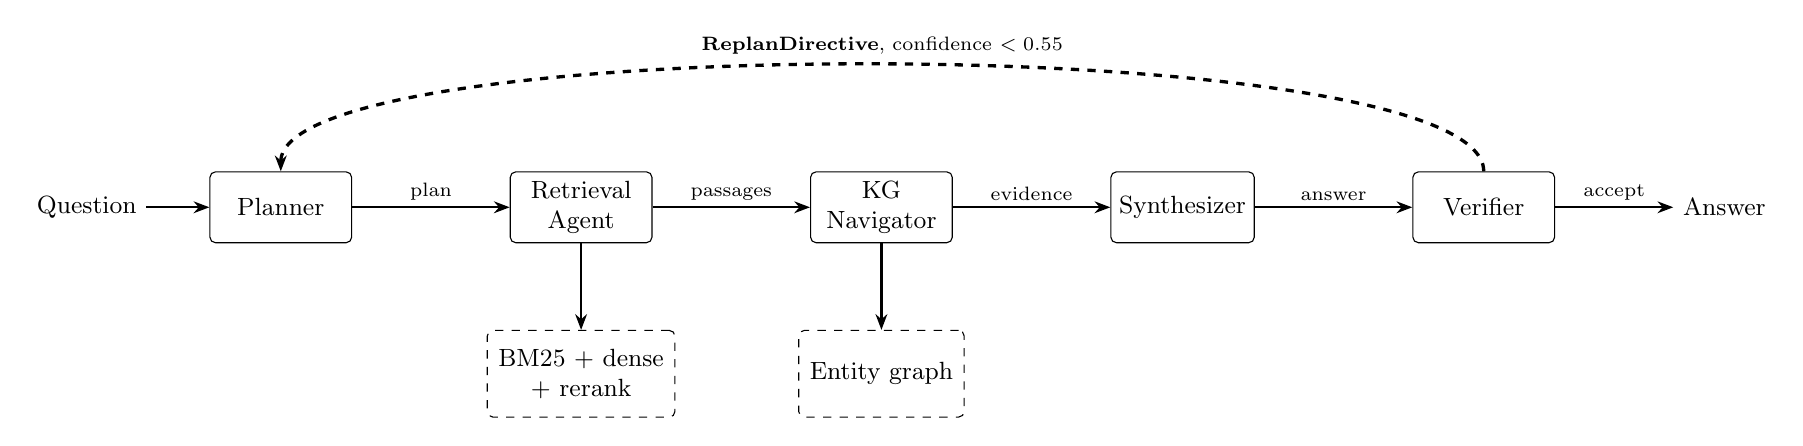
\begin{tikzpicture}[
    font=\small,
    box/.style={draw, rounded corners=2pt, minimum height=9mm,
                minimum width=18mm, align=center, inner sep=3pt},
    store/.style={draw, dashed, rounded corners=2pt, minimum height=11mm,
                  align=center, inner sep=4pt},
    flow/.style={-{Stealth[length=2mm]}, thick},
    back/.style={-{Stealth[length=2mm]}, very thick, dashed}
  ]
    \node (q) {Question};
    \node[box, right=8mm of q]     (plan) {Planner};
    \node[box, right=20mm of plan] (retr) {Retrieval\\Agent};
    \node[box, right=20mm of retr] (kg)   {KG\\Navigator};
    \node[box, right=20mm of kg]   (syn)  {Synthesizer};
    \node[box, right=20mm of syn]  (ver)  {Verifier};
    \node[right=15mm of ver]       (ans)  {Answer};

    \node[store, below=11mm of retr] (idx)   {BM25 $+$ dense\\$+$ rerank};
    \node[store, below=11mm of kg]   (graph) {Entity graph};

    \draw[flow] (q) -- (plan);
    \draw[flow] (plan) -- node[above, font=\scriptsize, inner sep=2pt] {plan} (retr);
    \draw[flow] (retr) -- node[above, font=\scriptsize, inner sep=2pt] {passages} (kg);
    \draw[flow] (kg)   -- node[above, font=\scriptsize, inner sep=2pt] {evidence} (syn);
    \draw[flow] (syn)  -- node[above, font=\scriptsize, inner sep=2pt] {answer} (ver);
    \draw[flow] (ver)  -- node[above, font=\scriptsize, inner sep=2pt] {accept} (ans);
    \draw[flow] (retr) -- (idx);
    \draw[flow] (kg)   -- (graph);

    \draw[back] (ver.north) .. controls +(0,18mm) and +(0,18mm) ..
      node[above, font=\scriptsize]
      {\textbf{ReplanDirective}, confidence $<0.55$} (plan.north);
  \end{tikzpicture}}
  \caption{The four-agent architecture. Solid arrows are the forward retrieval
  path; dashed boxes are offline artefacts. The dashed backward edge is the
  Verifier-to-Planner feedback loop, the only information that flows against
  the pipeline.}
  \label{fig:architecture}
\end{figure}

\subsection{Query Decomposition and Refinement}
\label{sec:decomposition}

The Planner converts a question into a directed acyclic graph of at most five
sub-queries. Each node carries its text, a dependency list, an intent and an
expected answer type, and may contain placeholders such as
\texttt{\{\{q1.answer\}\}}. Execution proceeds in topological order, and a
node's placeholders are substituted from its dependencies immediately before it
is routed, so the second-hop query is a genuinely different string at
retrieval time from the one the Planner emitted. This is the territory of
Self-Ask~\cite{press2023selfask} and IRCoT~\cite{trivedi2023interleaving},
with four differences. The plan is a validated data structure rather than a
decoding trajectory, and every mechanical repair is recorded. It is a graph,
so a comparison question yields two independent roots retrieved together.
Query expansion rides inside the same planner response, so it costs no
additional call. And the plan can be revised on evidence from a downstream
agent, which no single-pass trajectory can do.

Two decisions followed from measurement. The plan's \texttt{strategy} label is
derived from the shape of the validated graph and overwrites what the model
reported: on eight representative questions the model produced structurally
correct decompositions 8 times out of 8 and labelled the strategy
\texttt{single\_hop} in 7 of them. It builds the graph well and names it badly.
Separately, the model reliably emits a final combiner node restating the
question and depending on every other node; detecting and skipping it removes
a third of all retrieval on a three-node comparison plan.

The Planner degrades along a deterministic ladder rather than failing: a
comparison template, then a two-node bridge template, then an identity plan
routed to hybrid search with reranking. That floor is not the
\texttt{hybrid\_rerank} baseline, and the ablation grid of
Chapter~\ref{ch:implementation} shows why the distinction matters: an identity
plan still passes through synthesis and verification, so the system with the
Planner removed is a one-node agentic system that answers and cites, not a
ranker.

\subsection{Tool-Augmented Retrieval}
\label{sec:tools}

Seven tools are declared in a registry, four over the indexes and three over
the entity graph, and the description that documents each to a human is the
string injected into the selection prompt, so documentation and registry
cannot drift apart.

Selection among the retrieval tools is a seven-rule decision table over
features of the resolved sub-query: token count, quoted spans, capitalised
runs, out-of-vocabulary rate against the BM25 lexicon, minimum document
frequency among content terms, and whether the node has dependencies. A
planner hint is honoured first (R1); an out-of-vocabulary rate above 0.34
routes to dense search (R2); short quoted or proper-noun-dense queries (R3) and
queries containing a term of document frequency three or fewer (R4) route to
BM25, the Babycham case; dependent nodes (R5) and long or entity-free queries
(R6) route to hybrid; and a default row (R7) makes the table total.

One fact about the table changes what the argument is about. In the headline
HotpotQA run the Planner attached a hint to every one of the 854 sub-queries it
emitted, so R1 fired on all 575 routing decisions and R2 through R7 never
executed. All seven rules are implemented and tested; on this data six are
dead code. The planning call the system pays for anyway already carries a
per-node tool choice, and the table's contribution was to avoid asking the
model twice. The saving is real, but the claim that lexical rules decide as a
model would have decided is untested. Reinforcement learning would enter here
and does not, because the only reward derives from gold supporting facts that
exist solely in the evaluation data.

\subsection{Knowledge Graph Traversal}
\label{sec:kg-traversal}

The KG Navigator operates on the entity graph of
Section~\ref{sec:preprocessing}. Linking is an alias-trie longest match and
costs no model call. Traversal is bounded at two hops and twenty-five
neighbours, expanded in deterministic order of descending edge weight. The
highest-value operation is bidirectional breadth-first search: given two or
more linked seeds it expands from each and reports the meeting node as the
bridge entity. Applied to the Babycham example, the alias Accolade Wines
occurring in the Babycham passage is an edge by construction, so the bridge
entity the retrieval stack cannot surface by ranking is recovered by a graph
walk in milliseconds. This is the concrete sense in which traversal is not
decorative: it is a second, structurally different mechanism for the one
operation single-shot retrieval provably cannot perform.

Traversal is also the most explainable component, because the path is the
explanation: every edge stores the sentence asserting it, so a traversal
result is scored by the same metrics as a retrieved passage. The limits are
equally clear. The graph is induced from mention co-occurrence, and 23.2\% of
HotpotQA edges and 21.0\% of 2Wiki edges carry no label beyond
\texttt{mentions}, so it is a navigation aid rather than a knowledge base.

\subsection{Self-Reflective Validation}
\label{sec:verification}

The Verifier receives the Synthesizer's answer with the evidence pool and
decides whether it is supported. Cited identifiers that do not exist are
recorded as hallucinated citations and contribute no support. A natural
language inference model, \texttt{cross-encoder/nli-deberta-v3-base}, is run
with each cited sentence as premise and the answer sentence as hypothesis; the
Synthesizer emits that sentence as a separate field precisely so the hypothesis
is a well-formed declarative sentence. Two further signals are computed,
citation grounding and retrieval agreement, and the four combine as
\[
  \mathrm{conf} = 0.45\,\mathrm{nli} + 0.25\,\mathrm{citation}
                + 0.15\,\mathrm{retrieval} + 0.15\,\mathrm{llm},
\]
renormalised when the model term is absent. That term is gated: the
adjudication call is issued only when the confidence computed without it falls
inside $[0.40, 0.70]$, since confident acceptances and rejections cannot have
their verdict changed by it.

Above the threshold of 0.55 the verdict is accept. Below it, with re-plans
remaining, the Verifier emits a directive carrying what could not be
established, which sub-queries returned nothing useful, and the normalised
text of every sub-query already tried. Without that ban list an 8B model told
only that its previous attempt was insufficient reliably re-emits the same
decomposition and burns both re-plans for nothing. Below the threshold with no
re-plans left the verdict is abstain, a label rather than a refusal: the best
candidate is still returned. Answer selection at termination is the argument
maximising confidence over all cycles, ties broken toward the earlier answer,
so a bad re-plan cannot silently overwrite a good first attempt, and the error
taxonomy of Chapter~\ref{ch:implementation} contains explicit false-accept and
false-reject categories so the loop is falsifiable.

\section{The Role of the Language Model}
\label{sec:llm-role}

The language model is the component that generalises, and everything else
exists to keep the number of calls small. Three decisions genuinely require it:
mapping an unseen compound question onto a dependency structure, composing a
short answer from heterogeneous evidence, and adjudicating the narrow band
where the numeric signals disagree. Everything else is deterministic. The
worst case over a question is 15 calls against a cap of 20, with four to seven
typical, and two calls are reserved so synthesis and verification always run.

Serving the model locally shaped the method, not only the deployment. Prompt
length is a latency cost, which is why the re-plan prompt passes retrieved
titles rather than text. And \texttt{qwen3} is a hybrid reasoning model that
emits a \texttt{<think>} block by default: with thinking enabled and a
128-token cap it spent the entire budget on a 503-character reasoning block
and produced no answer at all. At that budget thinking starves the response,
so it is suppressed for the evaluated grid, and Section~\ref{sec:improvement}
reports what happens when it is switched back on for one agent with a budget
large enough to hold it.

\section{Architectural Summary}
\label{sec:arch-summary}

Read left to right, Figure~\ref{fig:architecture} is a pipeline; the dashed
edge, along which the Verifier returns a directive to the Planner below a
confidence of 0.55, is what makes it an agent. Every other component is
standard machinery arranged carefully, and Chapter~\ref{ch:implementation}
isolates that edge's effect by ablation.

\chapter{System Implementation and Evaluation}
\label{ch:implementation}

Chapter~\ref{ch:methodology} argued that a multi-hop need cannot be served by a
single retrieval round and set out the four agents that answer it. This chapter
describes how they are built, how the system is measured, and what the
measurements show. It closes with a bounded improvement loop, because a
negative result is more useful when the obvious remedies have been tried.

\section{System Architecture}
\label{sec:architecture}

The orchestrator is an explicit state machine rather than a chain of function
calls. Nine states, from \texttt{INIT} through \texttt{PLAN},
\texttt{EXECUTE}, \texttt{SYNTHESIZE} and \texttt{VERIFY} to \texttt{DONE},
and fifteen labelled transitions are enumerated in the source, and the
transition sequence each question took is written into its trace. This costs
more code than implicit control flow and buys inspectability: the claim that
the system re-plans is checkable against a recorded path, and every early exit
is attributable to a named guard.

Only one transition runs backwards. \texttt{REPLAN\_GATE} returns to
\texttt{PLAN} when the Verifier's confidence is below threshold. An agent that
can send work backwards can loop, so five guards are evaluated in order, on
the re-plan count, the iteration count, the remaining calls, the elapsed
time, and whether the directive names anything missing. A sixth check rejects
a revised plan whose sub-queries pair with the previous plan's at a Jaccard
similarity of 0.85 or above, because a local 8B model told its attempt was
insufficient will frequently re-emit the same decomposition in different
words.

\section{Implementation Details}
\label{sec:inference}

All generation runs on \texttt{qwen3:8b} at Q4\_K\_M quantisation through
Ollama on an RTX 5060 laptop GPU with 8\,GB of VRAM. Measured throughput is 52
tokens per second warm, and a schema-constrained planning call averages
3.75\,s. The card is effectively full: the model and its 8192-token context
occupy 6707 of 8151\,MiB, so the three sentence-transformer encoders run on
CPU at query time, where they cost well under a second per question. The
configuration file declares a response cache; none is implemented, so every
latency reported here is an uncached measurement.

Every agent calls the model with a JSON schema and parses the result through a
five-rung ladder ending in a re-prompt. Each question carries a budget of 20
calls, 6 iterations and 300\,s, checked and never raised as an exception, so
that running out of calls is distinguishable from crashing. Two calls are
reserved for synthesis and verification, so a planner that decomposes
aggressively cannot leave nothing with which to answer.

All results use the frozen 250-question samples of Section~\ref{sec:sampling}.
Every run writes a JSON Lines trace with one record per question, a metadata
file capturing the full configuration, library versions, model digest and
seed, and a flat metrics file. The harness checkpoints by appending, so a run
interrupted at question 194 resumes at 194. Sorting is deterministic with an
explicit tiebreaker on document identifier. The implementation is covered by
461 automated tests, three of which enforce properties that would otherwise
fail silently: no module outside the model client can reach the network, no
agent reads the gold answer, and the graph builder never opens a gold evidence
file.

\section{Baselines and Metrics}
\label{sec:baselines}

Five baselines run from weakest to strongest. \texttt{bm25\_only} and
\texttt{dense\_only} isolate the two channels. \texttt{hybrid\_rerank} fuses
them and reranks the top 50 with the cross-encoder on every question, with the
margin gate switched off so the baseline is not weakened. \texttt{naive\_rag}
retrieves once with the same pipeline and makes one generation call, so the
difference between it and \texttt{hybrid\_rerank} is one generation step and
nothing else. \texttt{self\_ask} is the published multi-hop
method~\cite{press2023selfask}: decomposition with no verification and no
re-planning, which makes the gap between it and the full system the closest
available estimate of what the backward edge is worth.

Three families of metric are reported together. Retrieval quality is
Recall@$\{2,5,10\}$, nDCG@10 and MRR, computed with \texttt{pytrec\_eval},
which wraps the same core as the evaluation that produced the published BEIR
figures~\cite{thakur2021beir}. Answer quality is exact match and token F1
under the official HotpotQA normalisation~\cite{yang2018hotpotqa}, with
supporting-fact EM and F1 over sentence identifiers. Agent-specific cost is
model calls, calls avoided by deterministic rules, tool calls, latency, plan
depth, re-plan rate and citation grounding. Reporting cost beside quality is
what the brief asks for and the only honest way to present an agentic system:
a method that gains three points of F1 for twenty times the compute has not
obviously won. Differences between systems are assessed with a paired
bootstrap over 1000 resamples of the identical question set.

\section{Results}
\label{sec:results}

% Chapter 4 -- main results
% GENERATED by src/agentic_ir/eval/tables.py -- do not edit by hand.
% Regenerate with: python -m agentic_ir.cli tables
% Requires \usepackage{booktabs} and \usepackage{graphicx};
% report/main.tex already loads both.
% Source runs:
%   hotpotqa/agentic_full: agentic_full_hotpotqa_20260904T221533Z (250 questions)
%   hotpotqa/agentic_no_kg: agentic_no_kg_hotpotqa_20260905T232702Z (250 questions)
%   hotpotqa/agentic_no_planner: agentic_no_planner_hotpotqa_20260905T224906Z (250 questions)
%   hotpotqa/agentic_no_verifier: agentic_no_verifier_hotpotqa_20260905T213927Z (250 questions)
%   hotpotqa/bm25_only: bm25_only_hotpotqa_20260902T113736Z (250 questions)
%   hotpotqa/dense_only: dense_only_hotpotqa_20260902T113746Z (250 questions)
%   hotpotqa/hybrid_rerank: hybrid_rerank_hotpotqa_20260902T114415Z (250 questions)
%   hotpotqa/naive_rag: naive_rag_hotpotqa_20260902T120313Z (250 questions)
%   hotpotqa/self_ask: self_ask_hotpotqa_20260904T194457Z (250 questions)
%   twowiki/agentic_full: agentic_full_twowiki_20260905T184526Z (250 questions)
%   twowiki/agentic_no_kg: agentic_no_kg_twowiki_20260906T124506Z (250 questions)
%   twowiki/agentic_no_planner: agentic_no_planner_twowiki_20260906T121324Z (250 questions)
%   twowiki/agentic_no_verifier: agentic_no_verifier_twowiki_20260906T103608Z (250 questions)
%   twowiki/bm25_only: bm25_only_twowiki_20260902T113905Z (250 questions)
%   twowiki/dense_only: dense_only_twowiki_20260902T113913Z (250 questions)
%   twowiki/hybrid_rerank: hybrid_rerank_twowiki_20260904T184235Z (250 questions)
%   twowiki/naive_rag: naive_rag_twowiki_20260904T201400Z (250 questions)
%   twowiki/self_ask: self_ask_twowiki_20260904T210355Z (250 questions)

\begin{table}[htbp]
  \centering
  \small
  \setlength{\tabcolsep}{4pt}
  \caption{Answer quality on \texttt{hotpotqa}, $n$ questions each. EM and F1 follow the official HotpotQA script; SP columns are set metrics over supporting-fact sentences. Reference system for the EM and F1 columns: \texttt{self\_ask}, marked $\dagger$. \textbf{Bold} = significantly better than the reference, $^{\downarrow}$ = significantly worse (paired bootstrap, 95\% CI of the paired difference excluding zero). Unmarked differences are not significant. SP-EM, SP-P, SP-R and SP-F1 are not one protocol: \texttt{agentic\_full}, \texttt{agentic\_no\_planner}, \texttt{agentic\_no\_kg} and \texttt{agentic\_no\_verifier} are scored on the sentences cited (mean 1.5 per question) and \texttt{bm25\_only}, \texttt{dense\_only}, \texttt{hybrid\_rerank}, \texttt{naive\_rag} and \texttt{self\_ask} on the whole evidence pool (mean 6.9), so no significance mark is placed between rows of different protocol; \textit{Pool SP-R} is scored the same way for every row. \texttt{--} across a whole row marks a configuration that has not been run. \texttt{bm25\_only}, \texttt{dense\_only} and \texttt{hybrid\_rerank} are retrieval-only: they emit a ranking and no answer, so the EM, F1 and $\Delta$F1 columns show \texttt{--} because there is no answer to score, not because the run is absent. Scoring the unattempted answer would report 0.000 and assert a failed attempt that never happened. $^{\ast}$ marks \texttt{naive\_rag} and \texttt{self\_ask}, whose citations do not resolve, so their supporting-fact scores are computed over the whole evidence pool rather than a cited subset.}
  \label{tab:main-answer-hotpotqa}
  \resizebox{\ifdim\width>\textwidth\textwidth\else\width\fi}{!}{%
  \begin{tabular}{lrrrcrrrrrr}
    \toprule
    System & $n$ & EM & F1 & F1 95\% CI & SP-EM & SP-P & SP-R & SP-F1 & Pool SP-R & $\Delta$F1 vs.\ ref.\ [95\% CI] \\
    \midrule
    \multicolumn{11}{@{}l}{\textit{Baselines (weakest first)}} \\
    \texttt{bm25\_only} & 250 & -- & -- & -- & 0.012 & 0.245$^{\downarrow}$ & 0.588$^{\downarrow}$ & 0.330$^{\downarrow}$ & 0.588$^{\downarrow}$ & -- \\
    \texttt{dense\_only} & 250 & -- & -- & -- & 0.020 & 0.283$^{\downarrow}$ & 0.650$^{\downarrow}$ & 0.377$^{\downarrow}$ & 0.650$^{\downarrow}$ & -- \\
    \texttt{hybrid\_rerank} & 250 & -- & -- & -- & 0.016 & 0.308$^{\dagger}$ & 0.706$^{\dagger}$ & 0.412$^{\dagger}$ & 0.706$^{\dagger}$ & -- \\
    \texttt{naive\_rag} & 250 & 0.496 & 0.581 & [0.522, 0.641] & 0.016$^{\ast}$ & 0.308$^{\ast}$ & 0.706$^{\ast}$ & 0.412$^{\ast}$ & 0.706 & -0.022 [-0.060, +0.018] \\
    \texttt{self\_ask} & 250 & 0.504$^{\dagger}$ & 0.603$^{\dagger}$ & [0.547, 0.659] & 0.016$^{\ast}$ & 0.302$^{\ast}$ & 0.696$^{\ast}$ & 0.405$^{\ast}$ & 0.696 & -- \\
    \addlinespace
    \multicolumn{11}{@{}l}{\textit{Agentic system and ablations}} \\
    \texttt{agentic\_full} & 250 & 0.432$^{\downarrow}$ & 0.510$^{\downarrow}$ & [0.451, 0.571] & 0.088 & 0.654 & 0.406 & 0.481 & \textbf{0.793} & -0.093 [-0.145, -0.039] \\
    \texttt{agentic\_no\_planner} & 250 & 0.456 & 0.543$^{\downarrow}$ & [0.489, 0.602] & 0.136 & 0.685 & 0.431 & 0.508 & \textbf{0.817} & -0.060 [-0.106, -0.009] \\
    \texttt{agentic\_no\_kg} & 250 & 0.404$^{\downarrow}$ & 0.501$^{\downarrow}$ & [0.443, 0.565] & 0.088 & 0.635 & 0.386 & 0.460 & \textbf{0.783} & -0.102 [-0.153, -0.051] \\
    \texttt{agentic\_no\_verifier} & 250 & 0.396$^{\downarrow}$ & 0.474$^{\downarrow}$ & [0.418, 0.536] & 0.108 & 0.672 & 0.414 & 0.491 & \textbf{0.795} & -0.130 [-0.185, -0.074] \\
    \bottomrule
  \end{tabular}}
\end{table}

\begin{table}[htbp]
  \centering
  \small
  \setlength{\tabcolsep}{4pt}
  \caption{Retrieval quality on \texttt{hotpotqa}, computed over the reciprocal-rank fusion of every sub-query's ranking against the gold supporting-fact documents. Reference system for the retrieval columns: \texttt{hybrid\_rerank}, marked $\dagger$. \textbf{Bold} = significantly better than the reference, $^{\downarrow}$ = significantly worse (paired bootstrap, 95\% CI of the paired difference excluding zero). Unmarked differences are not significant. \texttt{--} across a whole row marks a configuration that has not been run.}
  \label{tab:main-retrieval-hotpotqa}
  \resizebox{\ifdim\width>\textwidth\textwidth\else\width\fi}{!}{%
  \begin{tabular}{lrrrrcr}
    \toprule
    System & R@2 & R@5 & R@10 & nDCG@10 & nDCG@10 95\% CI & MRR \\
    \midrule
    \multicolumn{7}{@{}l}{\textit{Baselines (weakest first)}} \\
    \texttt{bm25\_only} & 0.576 & 0.700 & 0.774$^{\downarrow}$ & 0.728$^{\downarrow}$ & [0.696, 0.754] & 0.873 \\
    \texttt{dense\_only} & 0.652 & 0.762 & 0.816$^{\downarrow}$ & 0.787$^{\downarrow}$ & [0.756, 0.817] & 0.917 \\
    \texttt{hybrid\_rerank} & 0.696 & 0.824 & 0.876$^{\dagger}$ & 0.835$^{\dagger}$ & [0.810, 0.859] & 0.935 \\
    \texttt{naive\_rag} & 0.696 & 0.824 & 0.876 & 0.835 & [0.810, 0.859] & 0.935 \\
    \texttt{self\_ask} & 0.688 & 0.838 & \textbf{0.888} & 0.837 & [0.812, 0.860] & 0.929 \\
    \addlinespace
    \multicolumn{7}{@{}l}{\textit{Agentic system and ablations}} \\
    \texttt{agentic\_full} & 0.602 & 0.742 & 0.812$^{\downarrow}$ & 0.763$^{\downarrow}$ & [0.734, 0.791] & 0.899 \\
    \texttt{agentic\_no\_planner} & 0.686 & 0.820 & 0.872 & 0.831$^{\downarrow}$ & [0.804, 0.855] & 0.933 \\
    \texttt{agentic\_no\_kg} & 0.604 & 0.746 & 0.820$^{\downarrow}$ & 0.766$^{\downarrow}$ & [0.737, 0.793] & 0.897 \\
    \texttt{agentic\_no\_verifier} & 0.612 & 0.756 & 0.796$^{\downarrow}$ & 0.758$^{\downarrow}$ & [0.729, 0.786] & 0.888 \\
    \bottomrule
  \end{tabular}}
\end{table}

\begin{table}[htbp]
  \centering
  \small
  \setlength{\tabcolsep}{4pt}
  \caption{Answer quality on \texttt{twowiki}, $n$ questions each. EM and F1 follow the official HotpotQA script; SP columns are set metrics over supporting-fact sentences. Reference system for the EM and F1 columns: \texttt{self\_ask}, marked $\dagger$. \textbf{Bold} = significantly better than the reference, $^{\downarrow}$ = significantly worse (paired bootstrap, 95\% CI of the paired difference excluding zero). Unmarked differences are not significant. SP-EM, SP-P, SP-R and SP-F1 are not one protocol: \texttt{agentic\_full}, \texttt{agentic\_no\_planner}, \texttt{agentic\_no\_kg} and \texttt{agentic\_no\_verifier} are scored on the sentences cited (mean 1.5 per question) and \texttt{bm25\_only}, \texttt{dense\_only}, \texttt{hybrid\_rerank}, \texttt{naive\_rag} and \texttt{self\_ask} on the whole evidence pool (mean 8.9), so no significance mark is placed between rows of different protocol; \textit{Pool SP-R} is scored the same way for every row. \texttt{--} across a whole row marks a configuration that has not been run. \texttt{bm25\_only}, \texttt{dense\_only} and \texttt{hybrid\_rerank} are retrieval-only: they emit a ranking and no answer, so the EM, F1 and $\Delta$F1 columns show \texttt{--} because there is no answer to score, not because the run is absent. Scoring the unattempted answer would report 0.000 and assert a failed attempt that never happened. $^{\ast}$ marks \texttt{naive\_rag} and \texttt{self\_ask}, whose citations do not resolve, so their supporting-fact scores are computed over the whole evidence pool rather than a cited subset.}
  \label{tab:main-answer-twowiki}
  \resizebox{\ifdim\width>\textwidth\textwidth\else\width\fi}{!}{%
  \begin{tabular}{lrrrcrrrrrr}
    \toprule
    System & $n$ & EM & F1 & F1 95\% CI & SP-EM & SP-P & SP-R & SP-F1 & Pool SP-R & $\Delta$F1 vs.\ ref.\ [95\% CI] \\
    \midrule
    \multicolumn{11}{@{}l}{\textit{Baselines (weakest first)}} \\
    \texttt{bm25\_only} & 250 & -- & -- & -- & 0.008 & 0.208$^{\downarrow}$ & 0.551$^{\downarrow}$ & 0.273$^{\downarrow}$ & 0.551$^{\downarrow}$ & -- \\
    \texttt{dense\_only} & 250 & -- & -- & -- & 0.020 & 0.244 & 0.605 & 0.314 & 0.605 & -- \\
    \texttt{hybrid\_rerank} & 250 & -- & -- & -- & 0.016 & 0.255$^{\dagger}$ & 0.622$^{\dagger}$ & 0.327$^{\dagger}$ & 0.622$^{\dagger}$ & -- \\
    \texttt{naive\_rag} & 250 & 0.152$^{\downarrow}$ & 0.200$^{\downarrow}$ & [0.155, 0.246] & 0.016$^{\ast}$ & 0.255$^{\ast}$ & 0.622$^{\ast}$ & 0.327$^{\ast}$ & 0.622 & -0.110 [-0.160, -0.063] \\
    \texttt{self\_ask} & 250 & 0.264$^{\dagger}$ & 0.310$^{\dagger}$ & [0.259, 0.364] & 0.016$^{\ast}$ & 0.246$^{\ast}$ & 0.627$^{\ast}$ & 0.318$^{\ast}$ & 0.627 & -- \\
    \addlinespace
    \multicolumn{11}{@{}l}{\textit{Agentic system and ablations}} \\
    \texttt{agentic\_full} & 250 & 0.224 & 0.267 & [0.216, 0.321] & 0.124 & 0.558 & 0.367 & 0.421 & \textbf{0.684} & -0.043 [-0.100, +0.014] \\
    \texttt{agentic\_no\_planner} & 250 & 0.324 & \textbf{0.388} & [0.329, 0.443] & 0.144 & 0.678 & 0.422 & 0.495 & \textbf{0.678} & +0.078 [+0.021, +0.135] \\
    \texttt{agentic\_no\_kg} & 250 & 0.256 & 0.285 & [0.229, 0.339] & 0.132 & 0.578 & 0.363 & 0.425 & \textbf{0.679} & -0.025 [-0.079, +0.033] \\
    \texttt{agentic\_no\_verifier} & 250 & 0.216 & 0.266 & [0.218, 0.319] & 0.148 & 0.612 & 0.403 & 0.465 & \textbf{0.689} & -0.044 [-0.102, +0.014] \\
    \bottomrule
  \end{tabular}}
\end{table}

\begin{table}[htbp]
  \centering
  \small
  \setlength{\tabcolsep}{4pt}
  \caption{Retrieval quality on \texttt{twowiki}, computed over the reciprocal-rank fusion of every sub-query's ranking against the gold supporting-fact documents. Reference system for the retrieval columns: \texttt{hybrid\_rerank}, marked $\dagger$. \textbf{Bold} = significantly better than the reference, $^{\downarrow}$ = significantly worse (paired bootstrap, 95\% CI of the paired difference excluding zero). Unmarked differences are not significant. \texttt{--} across a whole row marks a configuration that has not been run.}
  \label{tab:main-retrieval-twowiki}
  \resizebox{\ifdim\width>\textwidth\textwidth\else\width\fi}{!}{%
  \begin{tabular}{lrrrrcr}
    \toprule
    System & R@2 & R@5 & R@10 & nDCG@10 & nDCG@10 95\% CI & MRR \\
    \midrule
    \multicolumn{7}{@{}l}{\textit{Baselines (weakest first)}} \\
    \texttt{bm25\_only} & 0.551 & 0.641 & 0.693$^{\downarrow}$ & 0.698$^{\downarrow}$ & [0.671, 0.724] & 0.910 \\
    \texttt{dense\_only} & 0.605 & 0.687 & 0.714 & 0.751 & [0.729, 0.774] & 0.981 \\
    \texttt{hybrid\_rerank} & 0.622 & 0.696 & 0.727$^{\dagger}$ & 0.756$^{\dagger}$ & [0.730, 0.780] & 0.967 \\
    \texttt{naive\_rag} & 0.622 & 0.696 & 0.727 & 0.756 & [0.730, 0.780] & 0.967 \\
    \texttt{self\_ask} & 0.627 & 0.756 & \textbf{0.797} & \textbf{0.790} & [0.765, 0.817] & 0.934 \\
    \addlinespace
    \multicolumn{7}{@{}l}{\textit{Agentic system and ablations}} \\
    \texttt{agentic\_full} & 0.559 & 0.683 & 0.727 & 0.723$^{\downarrow}$ & [0.697, 0.748] & 0.917 \\
    \texttt{agentic\_no\_planner} & 0.621 & 0.698 & 0.731 & 0.757 & [0.732, 0.781] & 0.967 \\
    \texttt{agentic\_no\_kg} & 0.571 & 0.685 & 0.736 & 0.732$^{\downarrow}$ & [0.707, 0.757] & 0.925 \\
    \texttt{agentic\_no\_verifier} & 0.566 & 0.684 & 0.719 & 0.721$^{\downarrow}$ & [0.696, 0.744] & 0.915 \\
    \bottomrule
  \end{tabular}}
\end{table}

% Chapter 4 -- agent-specific measures
% GENERATED by src/agentic_ir/eval/tables.py -- do not edit by hand.
% Regenerate with: python -m agentic_ir.cli tables
% Requires \usepackage{booktabs} and \usepackage{graphicx};
% report/main.tex already loads both.
% Source runs:
%   hotpotqa/agentic_full: agentic_full_hotpotqa_20260904T221533Z (250 questions)
%   hotpotqa/agentic_no_kg: agentic_no_kg_hotpotqa_20260905T232702Z (250 questions)
%   hotpotqa/agentic_no_planner: agentic_no_planner_hotpotqa_20260905T224906Z (250 questions)
%   hotpotqa/agentic_no_verifier: agentic_no_verifier_hotpotqa_20260905T213927Z (250 questions)
%   hotpotqa/bm25_only: bm25_only_hotpotqa_20260902T113736Z (250 questions)
%   hotpotqa/dense_only: dense_only_hotpotqa_20260902T113746Z (250 questions)
%   hotpotqa/hybrid_rerank: hybrid_rerank_hotpotqa_20260902T114415Z (250 questions)
%   hotpotqa/naive_rag: naive_rag_hotpotqa_20260902T120313Z (250 questions)
%   hotpotqa/self_ask: self_ask_hotpotqa_20260904T194457Z (250 questions)
%   twowiki/agentic_full: agentic_full_twowiki_20260905T184526Z (250 questions)
%   twowiki/agentic_no_verifier: agentic_no_verifier_twowiki_20260906T103608Z (16 questions)  PRELIMINARY: short of the 250-question evaluation slice; deltas and significance withheld
%   twowiki/bm25_only: bm25_only_twowiki_20260902T113905Z (250 questions)
%   twowiki/dense_only: dense_only_twowiki_20260902T113913Z (250 questions)
%   twowiki/hybrid_rerank: hybrid_rerank_twowiki_20260904T184235Z (250 questions)
%   twowiki/naive_rag: naive_rag_twowiki_20260904T201400Z (250 questions)
%   twowiki/self_ask: self_ask_twowiki_20260904T210355Z (250 questions)

\begin{table}[htbp]
  \centering
  \small
  \setlength{\tabcolsep}{4pt}
  \caption{Agent-specific cost on \texttt{hotpotqa}, per question. \textit{LLM calls} counts logical calls, cache hits included; \textit{Saved} counts calls a deterministic rule replaced, under the definition stated below; \textit{Re-plan rate} is a fraction of questions, not a mean count; \textit{Cite grounding} is averaged only over questions that produced a non-empty answer, so it cannot be inflated by abstentions. \textbf{Latency is the median per question, with the maximum beside it}, and every other column is a mean: latency is the one unbounded quantity here, so it is the one a single hung question can dominate, and a mean of it would report that question rather than the system. The maximum is printed rather than trimmed so the outlier stays in view. Latency is only comparable between cold-cache runs. \textbf{One or more questions overran the 300\,s \texttt{orchestrator.max\_wall\_clock\_s} budget}: \texttt{agentic\_full} (65744.3\,s on \texttt{5a7af32e55429931da12c99c}, 18.3\,h), \texttt{agentic\_no\_kg} (36447.4\,s on \texttt{5ae603ba5542996de7b71af4}, 10.1\,h). The budget is evidently only tested between state transitions, so it cannot pre-empt a call that blocks inside one; this is a system defect and not only a reporting one, and it is why the central column is a median. The arithmetic mean of \texttt{latency\_s} on such a run is that single question divided by $n$ and describes nothing that happens per question. See \texttt{docs/report-audit.md}. \textbf{\textit{Saved} is recomputed from the step trace under one definition}: a call is saved only when a deterministic rule produced an output that, absent the rule, this configuration would have obtained by an LLM call. The agents' own counter credits every rule that fired; two of those rules stand in for calls this configuration cannot make -- with \texttt{heuristic\_shortcut: true} the LLM router is unreachable for every sub-query, and with \texttt{entity\_linker: alias\_match} there is no LLM entity linker to skip -- and the identity plan of the no-planner ablation is the ablation itself, not a rule gating a planner call. A verifier skip for an empty or already-insufficient answer is a call nobody would make, not one replaced. The extraction ladder, which replaces a real rung-4 LLM call on every rung-1 to rung-3 success, never incremented the counter at all. Per-question decomposition, counted terms in bold, so any other definition can be applied from the same numbers: \texttt{agentic\_full}: routing 3.31, KG alias 2.54, \textbf{verifier gate 1.21}, verifier pointless 0.04, \textbf{extraction 1.39} (agents recorded 7.10); \texttt{agentic\_no\_planner}: routing 1.00, KG alias 0.94, \textbf{verifier gate 0.64}, verifier pointless 0.01, planner ablation 1.19 (agents recorded 3.78); \texttt{agentic\_no\_kg}: routing 3.28, \textbf{verifier gate 1.11}, verifier pointless 0.04, \textbf{extraction 1.40} (agents recorded 4.42); \texttt{agentic\_no\_verifier}: routing 2.26, KG alias 1.59, \textbf{extraction 1.16} (agents recorded 3.85). \textit{Plan depth} is the depth of the \textit{selected} plan (the cycle FINALIZE chose, \texttt{best\_cycle}), as \texttt{docs/architecture.md} \S6 defines it; the orchestrator's own metrics block records the \textit{latest} plan's depth and the two differ wherever a re-plan executed and the first cycle's answer was kept (\texttt{agentic\_full} 1.71 selected against 1.56 latest, \texttt{agentic\_no\_kg} 1.75 selected against 1.60 latest). \textit{Re-plan rate} is the fraction of questions on which the verifier triggered at least one re-plan (\textit{trig.}) and the fraction on which a re-planned cycle actually executed (\textit{exec.}); the two differ when the planner's re-plan was a near-duplicate of a plan already run and transition T2b discarded it, which the trace counts as a re-plan but not as a cycle. Questions with a discarded re-plan: \texttt{agentic\_full} (4 of 250 questions, executed rate 0.472), \texttt{agentic\_no\_planner} (47 of 250 questions, executed rate 0.000), \texttt{agentic\_no\_kg} (4 of 250 questions, executed rate 0.444). \texttt{--} across a whole row marks a configuration that has not been run.}
  \label{tab:agent-metrics-hotpotqa}
  \resizebox{\ifdim\width>\textwidth\textwidth\else\width\fi}{!}{%
  \begin{tabular}{lrrrrrrrrrr}
    \toprule
    System & LLM calls & Saved & Tool calls & Latency (s) med. & Latency (s) max & Plan depth & Sub-queries & Re-plan rate (trig.) & Re-plan rate (exec.) & Cite grounding \\
    \midrule
    \multicolumn{11}{@{}l}{\textit{Baselines (weakest first)}} \\
    \texttt{bm25\_only} & 0.00 & 0.00 & 1.00 & 0.0 & 0.0 & 1.00 & 1.00 & 0.000 & 0.000 & 0.000 \\
    \texttt{dense\_only} & 0.00 & 0.00 & 1.00 & 0.1 & 16.4 & 1.00 & 1.00 & 0.000 & 0.000 & 0.000 \\
    \texttt{hybrid\_rerank} & 0.00 & 0.00 & 2.00 & 4.9 & 36.8 & 1.00 & 1.00 & 0.000 & 0.000 & 0.000 \\
    \texttt{naive\_rag} & 1.00 & 0.00 & 2.00 & 8.7 & 31.5 & 1.00 & 1.00 & 0.000 & 0.000 & 0.000 \\
    \texttt{self\_ask} & 1.24 & 0.00 & 2.41 & 4.5 & 35.7 & 1.20 & 1.20 & 0.000 & 0.000 & 0.000 \\
    \addlinespace
    \multicolumn{11}{@{}l}{\textit{Agentic system and ablations}} \\
    \texttt{agentic\_full} & 4.26 & 2.60 & 14.83 & 28.3 & 65744.3 & 1.71 & 1.80 & 0.472 & 0.472 & 0.960 \\
    \texttt{agentic\_no\_planner} & 1.35 & 0.64 & 3.94 & 9.7 & 37.4 & 1.00 & 1.00 & 0.188 & 0.000 & 0.936 \\
    \texttt{agentic\_no\_kg} & 4.28 & 2.51 & 8.15 & 11.8 & 36447.4 & 1.75 & 1.84 & 0.444 & 0.444 & 0.968 \\
    \texttt{agentic\_no\_verifier} & 2.06 & 1.16 & 10.88 & 16.5 & 46.9 & 1.98 & 2.34 & 0.000 & 0.000 & 0.000 \\
    \bottomrule
  \end{tabular}}
\end{table}

\begin{table}[htbp]
  \centering
  \small
  \setlength{\tabcolsep}{4pt}
  \caption{Agent-specific cost on \texttt{twowiki}, per question. \textit{LLM calls} counts logical calls, cache hits included; \textit{Saved} counts calls a deterministic rule replaced, under the definition stated below; \textit{Re-plan rate} is a fraction of questions, not a mean count; \textit{Cite grounding} is averaged only over questions that produced a non-empty answer, so it cannot be inflated by abstentions. \textbf{Latency is the median per question, with the maximum beside it}, and every other column is a mean: latency is the one unbounded quantity here, so it is the one a single hung question can dominate, and a mean of it would report that question rather than the system. The maximum is printed rather than trimmed so the outlier stays in view. Latency is only comparable between cold-cache runs. \textbf{\textit{Saved} is recomputed from the step trace under one definition}: a call is saved only when a deterministic rule produced an output that, absent the rule, this configuration would have obtained by an LLM call. The agents' own counter credits every rule that fired; two of those rules stand in for calls this configuration cannot make -- with \texttt{heuristic\_shortcut: true} the LLM router is unreachable for every sub-query, and with \texttt{entity\_linker: alias\_match} there is no LLM entity linker to skip -- and the identity plan of the no-planner ablation is the ablation itself, not a rule gating a planner call. A verifier skip for an empty or already-insufficient answer is a call nobody would make, not one replaced. The extraction ladder, which replaces a real rung-4 LLM call on every rung-1 to rung-3 success, never incremented the counter at all. Per-question decomposition, counted terms in bold, so any other definition can be applied from the same numbers: \texttt{agentic\_full}: routing 3.68, KG alias 2.32, \textbf{verifier gate 1.16}, verifier pointless 0.03, \textbf{extraction 1.94} (agents recorded 7.19); \texttt{agentic\_no\_verifier}: routing 2.81, KG alias 1.69, \textbf{extraction 1.75} (agents recorded 4.50). \textit{Plan depth} is the depth of the \textit{selected} plan (the cycle FINALIZE chose, \texttt{best\_cycle}), as \texttt{docs/architecture.md} \S6 defines it; the orchestrator's own metrics block records the \textit{latest} plan's depth and the two differ wherever a re-plan executed and the first cycle's answer was kept (\texttt{agentic\_full} 1.90 selected against 1.76 latest). \textit{Re-plan rate} is the fraction of questions on which the verifier triggered at least one re-plan (\textit{trig.}) and the fraction on which a re-planned cycle actually executed (\textit{exec.}); the two differ when the planner's re-plan was a near-duplicate of a plan already run and transition T2b discarded it, which the trace counts as a re-plan but not as a cycle. Questions with a discarded re-plan: \texttt{agentic\_full} (3 of 250 questions, executed rate 0.392). \texttt{--} across a whole row marks a configuration that has not been run. \textbf{$^{\ddagger}$ marks a preliminary row}: \texttt{agentic\_no\_verifier} ($n=16$) had not covered the full 250-question evaluation slice when this table was generated, so the point estimates are over the questions completed so far and every delta, $p$-value and significance mark against it is withheld -- a paired test between a prefix and the full slice is not a paired test. These numbers will move; they are not final results.}
  \label{tab:agent-metrics-twowiki}
  \resizebox{\ifdim\width>\textwidth\textwidth\else\width\fi}{!}{%
  \begin{tabular}{lrrrrrrrrrr}
    \toprule
    System & LLM calls & Saved & Tool calls & Latency (s) med. & Latency (s) max & Plan depth & Sub-queries & Re-plan rate (trig.) & Re-plan rate (exec.) & Cite grounding \\
    \midrule
    \multicolumn{11}{@{}l}{\textit{Baselines (weakest first)}} \\
    \texttt{bm25\_only} & 0.00 & 0.00 & 1.00 & 0.0 & 0.0 & 1.00 & 1.00 & 0.000 & 0.000 & 0.000 \\
    \texttt{dense\_only} & 0.00 & 0.00 & 1.00 & 0.1 & 13.9 & 1.00 & 1.00 & 0.000 & 0.000 & 0.000 \\
    \texttt{hybrid\_rerank} & 0.00 & 0.00 & 2.00 & 8.3 & 27.0 & 1.00 & 1.00 & 0.000 & 0.000 & 0.000 \\
    \texttt{naive\_rag} & 1.00 & 0.00 & 2.00 & 12.2 & 29.7 & 1.00 & 1.00 & 0.000 & 0.000 & 0.000 \\
    \texttt{self\_ask} & 1.46 & 0.00 & 2.86 & 13.2 & 40.3 & 1.43 & 1.43 & 0.000 & 0.000 & 0.000 \\
    \addlinespace
    \multicolumn{11}{@{}l}{\textit{Agentic system and ablations}} \\
    \texttt{agentic\_full} & 3.80 & 3.10 & 16.00 & 35.4 & 121.5 & 1.90 & 2.26 & 0.392 & 0.392 & 0.976 \\
    \texttt{agentic\_no\_planner} & -- & -- & -- & -- & -- & -- & -- & -- & -- & -- \\
    \texttt{agentic\_no\_kg} & -- & -- & -- & -- & -- & -- & -- & -- & -- & -- \\
    \texttt{agentic\_no\_verifier}$^{\ddagger}$ & 2.00 & 1.75 & 12.38 & 11.6 & 21.9 & 2.12 & 2.81 & 0.000 & 0.000 & 0.000 \\
    \bottomrule
  \end{tabular}}
\end{table}


Tables~\ref{tab:main-answer-hotpotqa} and~\ref{tab:main-answer-twowiki}
report answer and supporting-fact quality,
Tables~\ref{tab:main-retrieval-hotpotqa} and~\ref{tab:main-retrieval-twowiki}
retrieval quality, and Tables~\ref{tab:agent-metrics-hotpotqa}
and~\ref{tab:agent-metrics-twowiki} the cost columns. Every figure is
generated from the run artefacts and inserted verbatim; no number in this
report is typed by hand from a run. A configuration that was not run renders
as a dash rather than as zero, and a retrieval-only system renders a dash in
the answer columns, because a zero there would assert a failed attempt that
never happened.

The retrieval ladder behaves as Chapter~\ref{ch:methodology} predicts. On
HotpotQA the sparse channel reaches Recall@10 of 0.774, the dense channel
0.816, and fusing them with reranking 0.876, six points over the better single
channel without any model involvement. Answer quality does not follow that
ladder, and the first thing to record is that the agentic system does not win.
On HotpotQA \texttt{self\_ask} reaches exact match 0.504 and F1 0.603,
\texttt{naive\_rag} 0.496 and 0.581, and \texttt{agentic\_full} 0.432 and
0.510. On 2WikiMultihopQA the leader is unchanged, \texttt{self\_ask} at 0.264
and 0.310 against \texttt{agentic\_full} at 0.224 and 0.267. Referenced to
\texttt{self\_ask}, the paired difference in F1 is $-0.093$ with a 95\%
interval of $[-0.145, -0.039]$ on HotpotQA, a deficit that is established, and
$-0.043$ $[-0.100, +0.014]$ on 2WikiMultihopQA, a consistent point estimate
that is not. On the answer string, decomposition with verification loses to
decomposition without it.

Retrieval shows the same deficit from the other side. \texttt{agentic\_full}
records nDCG@10 of 0.763 on HotpotQA against 0.835 for \texttt{hybrid\_rerank},
and 0.723 on 2WikiMultihopQA against 0.756, both significantly worse. The
reported ranking for a multi-hop configuration is the fusion of every
sub-query's list, and narrow sub-queries each relevant to one hop dilute the
head of the combined list. On 2WikiMultihopQA the two systems tie exactly on
Recall@10 at 0.727 while the agentic nDCG@10 is three points lower: the same
documents are found, further down, spread across several lists.

Supporting-fact F1 is the metric on which the trade is favourable, and it has
to be read with care. \texttt{agentic\_full} reaches 0.481 on HotpotQA against
0.412 for \texttt{hybrid\_rerank}, and 0.421 against 0.327 on 2WikiMultihopQA,
but the agentic rows are scored on the sentences the system cited, a mean of
1.5 per question, while the baselines are scored on their whole evidence pool,
a mean of 6.9 and 8.9. The two protocols trade precision against recall in
opposite directions and one F1 across them does not rank the systems; the
tables place no significance mark between rows of different protocol. The one
supporting-fact column scored the same way for every row is the recall of the
whole pool, and on it the agentic system leads every baseline: 0.793 against
0.706 on HotpotQA and 0.684 against 0.622 on 2WikiMultihopQA, both
significant. What is categorical is citation grounding: 0.960 and 0.976 for
\texttt{agentic\_full} and 0.000 for every baseline, whose citations resolve
to nothing. The defensible claim from this grid is about grounded and
auditable answers rather than accuracy: the system returns a somewhat worse
answer with a precise, machine-checkable account of itself.

The cost columns price that account. \texttt{agentic\_full} spends 4.26 model
calls per question on HotpotQA and 3.80 on 2WikiMultihopQA against 1.24 and
1.46 for \texttt{self\_ask}, and issues 14.83 and 16.00 tool calls against
2.41 and 2.86. Deterministic rules displace a real minority of the inference a
fully model-driven version would spend, 2.60 and 3.10 calls per question; they
do not displace more than the three reasoning agents consume. Latency is
printed as a median with the maximum beside it. On 2WikiMultihopQA the full
system costs a median of 35.4\,s against 13.2\,s for \texttt{self\_ask}; on
HotpotQA 28.3\,s against 4.5\,s, and the maximum is 65744\,s, 18.3 hours on one
question inside a single Synthesizer call. No arrangement of four model calls
consumes that; the host was almost certainly suspended with the call open. The
measurement identifies a defect in the budget itself: the 300\,s guard is
tested between nodes and before calls, never during one, so it cannot pre-empt
a call that blocks.

\section{Ablation Study}
\label{sec:ablations}

% Chapter 4 -- ablation study
% GENERATED by src/agentic_ir/eval/tables.py -- do not edit by hand.
% Regenerate with: python -m agentic_ir.cli tables
% Requires \usepackage{booktabs} and \usepackage{graphicx};
% report/main.tex already loads both.
% Source runs:
%   hotpotqa/agentic_full: agentic_full_hotpotqa_20260904T221533Z (250 questions)
%   hotpotqa/agentic_no_kg: agentic_no_kg_hotpotqa_20260905T232702Z (17 questions)  PRELIMINARY: short of the 250-question evaluation slice; deltas and significance withheld
%   hotpotqa/agentic_no_planner: agentic_no_planner_hotpotqa_20260905T224906Z (250 questions)
%   hotpotqa/agentic_no_verifier: agentic_no_verifier_hotpotqa_20260905T213927Z (250 questions)
%   hotpotqa/bm25_only: bm25_only_hotpotqa_20260902T113736Z (250 questions)
%   hotpotqa/dense_only: dense_only_hotpotqa_20260902T113746Z (250 questions)
%   hotpotqa/hybrid_rerank: hybrid_rerank_hotpotqa_20260902T114415Z (250 questions)
%   hotpotqa/naive_rag: naive_rag_hotpotqa_20260902T120313Z (250 questions)
%   hotpotqa/self_ask: self_ask_hotpotqa_20260904T194457Z (250 questions)
%   twowiki/agentic_full: agentic_full_twowiki_20260905T184526Z (250 questions)
%   twowiki/bm25_only: bm25_only_twowiki_20260902T113905Z (250 questions)
%   twowiki/dense_only: dense_only_twowiki_20260902T113913Z (250 questions)
%   twowiki/hybrid_rerank: hybrid_rerank_twowiki_20260904T184235Z (250 questions)
%   twowiki/naive_rag: naive_rag_twowiki_20260904T201400Z (250 questions)
%   twowiki/self_ask: self_ask_twowiki_20260904T210355Z (250 questions)

\begin{table}[htbp]
  \centering
  \small
  \setlength{\tabcolsep}{4pt}
  \caption{Ablation study on \texttt{hotpotqa}. Deltas are measured against \texttt{agentic\_full} ($\dagger$), so a \textit{negative} $\Delta$F1 means the removed component was helping. \textbf{Bold} marks an ablation significantly \textit{better} than the full system and $^{\downarrow}$ one significantly worse (paired bootstrap, 95\% CI of the difference excluding zero); unmarked differences are not significant. Sample sizes are stated per row and are not assumed equal: \texttt{agentic\_full} $n=250$, \texttt{agentic\_no\_planner} $n=250$, \texttt{agentic\_no\_kg} $n=17^{\ddagger}$, \texttt{agentic\_no\_verifier} $n=250$, \texttt{hybrid\_rerank} $n=250$, against a 250-question evaluation slice. \texttt{hybrid\_rerank} is repeated from the main results as the non-agentic floor, since removing planning, synthesis and verification reduces the pipeline to it. Latency is the median per question, matching Table~\ref{tab:agent-metrics-hotpotqa}; the maximum and the wall-clock overruns are reported there. \texttt{--} across a whole row marks a configuration that has not been run. \texttt{hybrid\_rerank} is retrieval-only: it emits a ranking and no answer, so the EM, F1, $\Delta$F1 and $p$ columns show \texttt{--} because there is no answer to score, not because the run is absent. Scoring the unattempted answer would report 0.000 and assert a failed attempt that never happened. \textbf{$^{\ddagger}$ marks a preliminary row}: \texttt{agentic\_no\_kg} ($n=17$) had not covered the full 250-question evaluation slice when this table was generated, so the point estimates are over the questions completed so far and every delta, $p$-value and significance mark against it is withheld -- a paired test between a prefix and the full slice is not a paired test. These numbers will move; they are not final results.}
  \label{tab:ablations-hotpotqa}
  \resizebox{\ifdim\width>\textwidth\textwidth\else\width\fi}{!}{%
  \begin{tabular}{lrrrrrrr}
    \toprule
    System & $n$ & EM & F1 & $\Delta$F1 vs.\ full [95\% CI] & $p$ & LLM calls & Latency (s) med. \\
    \midrule
    \texttt{agentic\_full} & 250 & 0.432$^{\dagger}$ & 0.510$^{\dagger}$ & -- & -- & 4.26 & 28.3 \\
    \texttt{agentic\_no\_planner} & 250 & 0.456 & 0.543 & +0.033 [-0.017, +0.086] & 0.186 & 1.35 & 9.7 \\
    \texttt{agentic\_no\_kg} & 17$^{\ddagger}$ & 0.471 & 0.565 & -- & -- & 3.53 & 10.6 \\
    \texttt{agentic\_no\_verifier} & 250 & 0.396$^{\downarrow}$ & 0.474$^{\downarrow}$ & -0.037 [-0.065, -0.011] & 0.008 & 2.06 & 16.5 \\
    \texttt{hybrid\_rerank} \textit{(non-agentic floor)} & 250 & -- & -- & -- & -- & 0.00 & 4.9 \\
    \bottomrule
  \end{tabular}}
\end{table}

\begin{table}[htbp]
  \centering
  \small
  \setlength{\tabcolsep}{4pt}
  \caption{Ablation study on \texttt{twowiki}. Deltas are measured against \texttt{agentic\_full} ($\dagger$), so a \textit{negative} $\Delta$F1 means the removed component was helping. \textbf{Bold} marks an ablation significantly \textit{better} than the full system and $^{\downarrow}$ one significantly worse (paired bootstrap, 95\% CI of the difference excluding zero); unmarked differences are not significant. Every row covers the same frozen 250-question evaluation slice as the main results -- no ablation was run on a reduced subsample (\texttt{agentic\_full} $n=250$, \texttt{hybrid\_rerank} $n=250$). \texttt{hybrid\_rerank} is repeated from the main results as the non-agentic floor, since removing planning, synthesis and verification reduces the pipeline to it. Latency is the median per question, matching Table~\ref{tab:agent-metrics-twowiki}; the maximum and the wall-clock overruns are reported there. \texttt{--} across a whole row marks a configuration that has not been run. \texttt{hybrid\_rerank} is retrieval-only: it emits a ranking and no answer, so the EM, F1, $\Delta$F1 and $p$ columns show \texttt{--} because there is no answer to score, not because the run is absent. Scoring the unattempted answer would report 0.000 and assert a failed attempt that never happened.}
  \label{tab:ablations-twowiki}
  \resizebox{\ifdim\width>\textwidth\textwidth\else\width\fi}{!}{%
  \begin{tabular}{lrrrrrrr}
    \toprule
    System & $n$ & EM & F1 & $\Delta$F1 vs.\ full [95\% CI] & $p$ & LLM calls & Latency (s) med. \\
    \midrule
    \texttt{agentic\_full} & 250 & 0.224$^{\dagger}$ & 0.267$^{\dagger}$ & -- & -- & 3.80 & 35.4 \\
    \texttt{agentic\_no\_planner} & -- & -- & -- & -- & -- & -- & -- \\
    \texttt{agentic\_no\_kg} & -- & -- & -- & -- & -- & -- & -- \\
    \texttt{agentic\_no\_verifier} & -- & -- & -- & -- & -- & -- & -- \\
    \texttt{hybrid\_rerank} \textit{(non-agentic floor)} & 250 & -- & -- & -- & -- & 0.00 & 8.3 \\
    \bottomrule
  \end{tabular}}
\end{table}


Three ablations attribute the behaviour to its parts
(Tables~\ref{tab:ablations-hotpotqa} and~\ref{tab:ablations-twowiki}), each
over the same 250 questions so every delta is paired.

\textbf{The verifier.} This is the measurement the project exists to make.
With the backward edge removed and everything else fixed, HotpotQA exact match
falls from 0.432 to 0.396 and F1 from 0.510 to 0.474, a paired $\Delta$F1 of
$-0.037$ $[-0.065, -0.011]$, $p = 0.008$. The loop pays for itself on this
dataset, at roughly double the model calls (4.26 against 2.06) and the median
latency (28.3\,s against 16.5\,s). Then 2WikiMultihopQA does not agree.
\texttt{agentic\_no\_verifier} scores 0.216 and 0.266 against the full
system's 0.224 and 0.267, a $\Delta$F1 of $-0.001$ $[-0.025, +0.025]$,
$p = 1.000$. It is not a failure to fire: the loop ran on 98 of 250 questions
and a later cycle was selected on 64, and it charged the same doubled cost for
a change of one thousandth of an F1 point. The honest statement is the
conditional one. The backward edge helps on HotpotQA and not on
2WikiMultihopQA, and one more dataset would not make it a general result. Two
readings fit: a system at F1 0.267 is failing for reasons a second attempt at
the same corpus cannot repair, and 2WikiMultihopQA's comparison templates
defeat an entailment check that reads one answer sentence, since ``A was born
before B'' is entailed by neither operand's page alone. The ablated system
being better attributed there, supporting-fact F1 0.465 against 0.421,
supports the second.

\textbf{The planner.} This is the surprise, and the project's most
consequential negative result. \texttt{agentic\_no\_planner} scores above the
full system on HotpotQA, exact match 0.456 and F1 0.543 against 0.432 and
0.510, $\Delta$F1 $+0.033$ $[-0.017, +0.086]$, not significant, at 1.35 model
calls and a median of 9.7\,s. On 2WikiMultihopQA it is decisive: 0.324 and
0.388 against 0.224 and 0.267, $\Delta$F1 $+0.121$ $[+0.067, +0.173]$,
$p < 0.001$, at 1.26 calls against 3.80 and 4.5\,s against 35.4\,s. Removing
the component the brief lists first is worth twelve F1 points on the harder
dataset at a third of the calls and an eighth of the wall clock, and the same
row is the only configuration in the grid to beat \texttt{self\_ask}
significantly, $\Delta$F1 $+0.078$ $[+0.021, +0.135]$, while grounding 0.900
of its citations. What that configuration is matters. With the Planner removed
the plan is one identity node, so it issues a single query exactly as
\texttt{naive\_rag} does, and \texttt{naive\_rag} scores 0.152 and 0.200 on
the same questions. The gap between two systems that each ask one question is
the rest of the agentic stack: graph evidence beside the retrieved passages,
sentence-granular pooling, synthesis constrained to cite what it used, and a
verification pass. The evidence handling earns its cost; the decomposition was
spending it. The cost grows with chain length, which rules out the reading
that decomposition merely dilutes a good ranking, since 2WikiMultihopQA's
rankings are the worse of the two. What grows with chain length is the number
of sub-answers an 8B model must compose across, and each composition is a
chance to lose the thread.

\textbf{The graph.} A null was always plausible, since the induced graph is a
navigation aid rather than a knowledge base, and a null is what returns.
\texttt{agentic\_no\_kg} scores 0.404 and 0.501 on HotpotQA, $\Delta$F1
$-0.009$ $[-0.048, +0.029]$, and 0.256 and 0.285 on 2WikiMultihopQA,
$\Delta$F1 $+0.018$ $[-0.015, +0.053]$, with retrieval statistically
indistinguishable from the full system's. What the graph changes is the bill:
tool calls fall from 14.83 to 8.15 per question and median latency from
28.3\,s to 11.8\,s on HotpotQA, mirrored on 2WikiMultihopQA. The KG Navigator
accounts for roughly half the system's tool calls and more than half its
latency and returns nothing either evaluation can detect. Unlike the planner
this is a null rather than a harm: the graph is paid for and ignored.

\section{Error Analysis}
\label{sec:errors}

% Chapter 4 -- error analysis
% GENERATED by src/agentic_ir/eval/tables.py -- do not edit by hand.
% Regenerate with: python -m agentic_ir.cli tables
% Requires \usepackage{booktabs} and \usepackage{graphicx};
% report/main.tex already loads both.
% Source runs:
%   hotpotqa/agentic_full: agentic_full_hotpotqa_20260904T221533Z (250 questions)
%   hotpotqa/agentic_no_kg: agentic_no_kg_hotpotqa_20260905T232702Z (250 questions)
%   hotpotqa/agentic_no_planner: agentic_no_planner_hotpotqa_20260905T224906Z (250 questions)
%   hotpotqa/agentic_no_verifier: agentic_no_verifier_hotpotqa_20260905T213927Z (250 questions)
%   hotpotqa/bm25_only: bm25_only_hotpotqa_20260902T113736Z (250 questions)
%   hotpotqa/dense_only: dense_only_hotpotqa_20260902T113746Z (250 questions)
%   hotpotqa/hybrid_rerank: hybrid_rerank_hotpotqa_20260902T114415Z (250 questions)
%   hotpotqa/naive_rag: naive_rag_hotpotqa_20260902T120313Z (250 questions)
%   hotpotqa/self_ask: self_ask_hotpotqa_20260904T194457Z (250 questions)
%   twowiki/agentic_full: agentic_full_twowiki_20260905T184526Z (250 questions)
%   twowiki/agentic_no_verifier: agentic_no_verifier_twowiki_20260906T103608Z (16 questions)  PRELIMINARY: short of the 250-question evaluation slice; deltas and significance withheld
%   twowiki/bm25_only: bm25_only_twowiki_20260902T113905Z (250 questions)
%   twowiki/dense_only: dense_only_twowiki_20260902T113913Z (250 questions)
%   twowiki/hybrid_rerank: hybrid_rerank_twowiki_20260904T184235Z (250 questions)
%   twowiki/naive_rag: naive_rag_twowiki_20260904T201400Z (250 questions)
%   twowiki/self_ask: self_ask_twowiki_20260904T210355Z (250 questions)

\begin{table}[htbp]
  \centering
  \small
  \setlength{\tabcolsep}{4pt}
  \caption{Failure profile on \texttt{hotpotqa}. Labels are assigned post hoc by \texttt{eval/error\_analysis.py} from the trace and the gold supporting facts -- deterministically, first match wins -- in a cascade from ``the system never had a chance'' to ``it had everything it needed and still got it wrong''. \texttt{verifier\_false\_accept} and \texttt{verifier\_false\_reject} are counted again in the totals, independently of the cascade: the ordered label makes a false reject nearly unreachable, and it is the count that makes the Verifier$\rightarrow$Planner loop falsifiable. Corpus titles were loaded, so the \texttt{decomposition\_error} rule's ``gold facts exist in the corpus'' clause is checked rather than assumed. A configuration with no run has no column. \texttt{bm25\_only}, \texttt{dense\_only} and \texttt{hybrid\_rerank} emit no answer at all, so their \textit{Correct} is structurally $0$ and every question is counted as an error; the informative rows for them are the retrieval labels, not the accuracy.}
  \label{tab:error-analysis-hotpotqa}
  \resizebox{\ifdim\width>\textwidth\textwidth\else\width\fi}{!}{%
  \begin{tabular}{lrrrrrrrrr}
    \toprule
    Label & \texttt{bm25\_only} & \texttt{dense\_only} & \texttt{hybrid\_rerank} & \texttt{naive\_rag} & \texttt{self\_ask} & \texttt{agentic\_full} & \texttt{agentic\_no\_planner} & \texttt{agentic\_no\_kg} & \texttt{agentic\_no\_verifier} \\
    \midrule
    \multicolumn{10}{@{}l}{\textit{Failure labels: count (share of all questions)}} \\
    \texttt{parse\_failure} & 0 (0.000) & 0 (0.000) & 0 (0.000) & 0 (0.000) & 0 (0.000) & 0 (0.000) & 0 (0.000) & 1 (0.004) & 0 (0.000) \\
    \texttt{budget\_exhausted} & 0 (0.000) & 0 (0.000) & 0 (0.000) & 0 (0.000) & 0 (0.000) & 0 (0.000) & 0 (0.000) & 0 (0.000) & 0 (0.000) \\
    \texttt{retrieval\_miss} & 4 (0.016) & 5 (0.020) & 0 (0.000) & 0 (0.000) & 0 (0.000) & 3 (0.012) & 1 (0.004) & 3 (0.012) & 3 (0.012) \\
    \texttt{decomposition\_error} & 105 (0.420) & 82 (0.328) & 62 (0.248) & 44 (0.176) & 31 (0.124) & 16 (0.064) & 46 (0.184) & 15 (0.060) & 3 (0.012) \\
    \texttt{bridge\_link\_failure} & 104 (0.416) & 115 (0.460) & 138 (0.552) & 55 (0.220) & 69 (0.276) & 17 (0.068) & 63 (0.252) & 15 (0.060) & 20 (0.080) \\
    \texttt{synthesis\_error} & 17 (0.068) & 42 (0.168) & 33 (0.132) & 19 (0.076) & 16 (0.064) & 57 (0.228) & 23 (0.092) & 60 (0.240) & 61 (0.244) \\
    \texttt{verifier\_false\_accept} & 0 (0.000) & 0 (0.000) & 0 (0.000) & 0 (0.000) & 0 (0.000) & 33 (0.132) & 0 (0.000) & 36 (0.144) & 0 (0.000) \\
    \texttt{verifier\_false\_reject} & 0 (0.000) & 0 (0.000) & 0 (0.000) & 0 (0.000) & 0 (0.000) & 0 (0.000) & 0 (0.000) & 1 (0.004) & 0 (0.000) \\
    \addlinespace
    \multicolumn{10}{@{}l}{\textit{Totals}} \\
    Questions scored & 250 & 250 & 250 & 250 & 250 & 250 & 250 & 250 & 250 \\
    Correct & 0 & 0 & 0 & 124 & 126 & 108 & 114 & 101 & 99 \\
    Accuracy & 0.000 & 0.000 & 0.000 & 0.496 & 0.504 & 0.432 & 0.456 & 0.404 & 0.396 \\
    Errors & 250 & 250 & 250 & 126 & 124 & 142 & 136 & 149 & 151 \\
    Errors with no rule firing & 20 & 6 & 17 & 8 & 8 & 16 & 3 & 18 & 64 \\
    Verifier false accepts & 0 & 0 & 0 & 0 & 0 & 92 & 74 & 99 & 0 \\
    Verifier false rejects & 0 & 0 & 0 & 0 & 0 & 2 & 0 & 5 & 0 \\
    Recoverable (some cycle was right) & 0 & 0 & 0 & 0 & 0 & 2 & 0 & 5 & 0 \\
    \bottomrule
  \end{tabular}}
\end{table}

\begin{table}[htbp]
  \centering
  \small
  \setlength{\tabcolsep}{4pt}
  \caption{Failure profile on \texttt{twowiki}. Labels are assigned post hoc by \texttt{eval/error\_analysis.py} from the trace and the gold supporting facts -- deterministically, first match wins -- in a cascade from ``the system never had a chance'' to ``it had everything it needed and still got it wrong''. \texttt{verifier\_false\_accept} and \texttt{verifier\_false\_reject} are counted again in the totals, independently of the cascade: the ordered label makes a false reject nearly unreachable, and it is the count that makes the Verifier$\rightarrow$Planner loop falsifiable. Corpus titles were loaded, so the \texttt{decomposition\_error} rule's ``gold facts exist in the corpus'' clause is checked rather than assumed. A configuration with no run has no column. \texttt{bm25\_only}, \texttt{dense\_only} and \texttt{hybrid\_rerank} emit no answer at all, so their \textit{Correct} is structurally $0$ and every question is counted as an error; the informative rows for them are the retrieval labels, not the accuracy. \textbf{$^{\ddagger}$ marks a preliminary row}: \texttt{agentic\_no\_verifier} ($n=16$) had not covered the full 250-question evaluation slice when this table was generated, so the point estimates are over the questions completed so far and every delta, $p$-value and significance mark against it is withheld -- a paired test between a prefix and the full slice is not a paired test. These numbers will move; they are not final results.}
  \label{tab:error-analysis-twowiki}
  \resizebox{\ifdim\width>\textwidth\textwidth\else\width\fi}{!}{%
  \begin{tabular}{lrrrrrrr}
    \toprule
    Label & \texttt{bm25\_only} & \texttt{dense\_only} & \texttt{hybrid\_rerank} & \texttt{naive\_rag} & \texttt{self\_ask} & \texttt{agentic\_full} & \texttt{agentic\_no\_verifier}$^{\ddagger}$ \\
    \midrule
    \multicolumn{8}{@{}l}{\textit{Failure labels: count (share of all questions)}} \\
    \texttt{parse\_failure} & 0 (0.000) & 0 (0.000) & 0 (0.000) & 0 (0.000) & 0 (0.000) & 0 (0.000) & 0 (0.000) \\
    \texttt{budget\_exhausted} & 0 (0.000) & 0 (0.000) & 0 (0.000) & 0 (0.000) & 0 (0.000) & 0 (0.000) & 0 (0.000) \\
    \texttt{retrieval\_miss} & 4 (0.016) & 0 (0.000) & 1 (0.004) & 1 (0.004) & 1 (0.004) & 1 (0.004) & 0 (0.000) \\
    \texttt{decomposition\_error} & 147 (0.588) & 144 (0.576) & 138 (0.552) & 124 (0.496) & 48 (0.192) & 22 (0.088) & 0 (0.000) \\
    \texttt{bridge\_link\_failure} & 45 (0.180) & 49 (0.196) & 50 (0.200) & 42 (0.168) & 81 (0.324) & 7 (0.028) & 1 (0.062) \\
    \texttt{synthesis\_error} & 36 (0.144) & 45 (0.180) & 46 (0.184) & 34 (0.136) & 19 (0.076) & 59 (0.236) & 2 (0.125) \\
    \texttt{verifier\_false\_accept} & 0 (0.000) & 0 (0.000) & 0 (0.000) & 0 (0.000) & 0 (0.000) & 82 (0.328) & 0 (0.000) \\
    \texttt{verifier\_false\_reject} & 0 (0.000) & 0 (0.000) & 0 (0.000) & 0 (0.000) & 0 (0.000) & 0 (0.000) & 0 (0.000) \\
    \addlinespace
    \multicolumn{8}{@{}l}{\textit{Totals}} \\
    Questions scored & 250 & 250 & 250 & 250 & 250 & 250 & 16 \\
    Correct & 0 & 0 & 0 & 38 & 66 & 56 & 2 \\
    Accuracy & 0.000 & 0.000 & 0.000 & 0.152 & 0.264 & 0.224 & 0.125 \\
    Errors & 250 & 250 & 250 & 212 & 184 & 194 & 14 \\
    Errors with no rule firing & 18 & 12 & 15 & 11 & 35 & 23 & 11 \\
    Verifier false accepts & 0 & 0 & 0 & 0 & 0 & 154 & 0 \\
    Verifier false rejects & 0 & 0 & 0 & 0 & 0 & 5 & 0 \\
    Recoverable (some cycle was right) & 0 & 0 & 0 & 0 & 0 & 5 & 0 \\
    \bottomrule
  \end{tabular}}
\end{table}


Failures are categorised from the traces against the gold supporting facts,
first match winning (Tables~\ref{tab:error-analysis-hotpotqa}
and~\ref{tab:error-analysis-twowiki}). Neither dataset records a single parse
failure or budget exhaustion in any configuration, which retires two concerns
the design spent effort on. Against \texttt{hybrid\_rerank},
\texttt{agentic\_full} reduces the share of questions labelled decomposition
error from 0.248 to 0.064 on HotpotQA and from 0.552 to 0.088 on
2WikiMultihopQA, and bridge-link failure from 0.552 to 0.068 and 0.200 to
0.028. Those are the two classes Chapter~\ref{ch:introduction} argued a
single-shot ranker cannot address, and they have very largely gone. What
replaces them is synthesis error, at 0.228 and 0.236, the dominant agentic
failure mode and more than three times the rate for \texttt{self\_ask}. The
system finds the right evidence and composes the wrong string from it.

The Verifier's behaviour is the other half of that picture. The traces record
92 false accepts on HotpotQA and 154 on 2WikiMultihopQA against 2 and 5 false
rejects. The loop is far too permissive, and the confidence signal is why: a
post-hoc sweep over the calibration slice finds an area under the ROC curve of
0.633 and an expected calibration error of 0.332, a usable ranking cut-point
and an unusable probability. The cleanest single failure is HotpotQA question
\texttt{5a7af32e55429931da12c99c}: the system answered New York City where the
gold is Brooklyn, New York, with an answer sentence copied from an unrelated
evidence sentence, and the Verifier scored entailment above 0.99 because a
copied sentence is trivially entailed by its source. The architecture entails
the answer sentence and never the answer string, and the two can come apart.

\section{Discussion}
\label{sec:discussion}

The grid does not support the claim this project would have preferred to make.
Agency did not buy accuracy. A published decomposition method with no
verification answers more questions correctly than the four-agent system at a
third of the calls, and the fused ranking the agentic system produces is
significantly worse than a single reranked query. Agency did buy grounded,
auditable answers, and the failure profile says where the effort belongs: not
in more planning, more traversal or more retrieval, all of which already
deliver the evidence, but in synthesis, where the right sentences become the
wrong span. A practitioner should take the following. For a ranked list, use
\texttt{hybrid\_rerank}. For a short answer where cost matters, use
\texttt{self\_ask}. The four-agent system earns its cost only where the answer
must be attributable. And the one-node configuration that deletes the Planner
is the system to start from, because it gives up nothing.

\section{Improving the System, and What It Cost}
\label{sec:improvement}

That last sentence was the starting point for a bounded improvement loop:
five hypotheses fixed in advance, each measured on the same frozen 250
questions and kept or dropped on a paired interval, under stop conditions
stated before any ran. One local model, no paid API, and the nine evaluated
configurations were not to change: every modification ships behind a flag
defaulting to the evaluated behaviour, and the four evaluated agentic
configurations are checked to resolve to identical settings before and after,
so \texttt{agentic\_full} remains the system this chapter describes. One
hypothesis survived.

\subsection{The Kept Change}

\texttt{qwen3:8b} is a hybrid reasoning model whose reasoning mode is
suppressed throughout the grid, for the reason Section~\ref{sec:llm-role}
gave. The kept configuration, \texttt{agentic\_v2}, re-enables it for exactly
one agent. The synthesiser reasons; the Planner, Retrieval Agent, KG Navigator
and Verifier do not, through a per-agent routing list added beside the global
flag. The configuration also raises the completion budget from 1024 to 5120
tokens, and that is part of the change: at 1024 the reasoning block consumes
the whole budget and the synthesiser returns nothing. It builds on the
one-node plan, since the ablation above showed decomposition subtracting from
the answer.

% GENERATED by src/agentic_ir/eval/tables.py::write_v2_tables -- do not edit by hand.
% Source runs: results/runs_v2 (the improvement loop). `cli tables` neither
% writes nor reads these -- discover_runs cannot see that directory, which is
% what keeps the report's nine-system grid exactly nine systems.
% Requires \usepackage{booktabs} and \usepackage{graphicx}.

\begin{table}[htbp]
  \centering
  \small
  \setlength{\tabcolsep}{4pt}
  \caption{The improvement loop's kept configuration against the reported system, its own base, and the strongest answer baseline. Paired on question id over the same frozen 250-question slice. Five of the six intervals exclude zero; the exception is \texttt{self\_ask} on HotpotQA, where the kept configuration ties a single-model baseline that has no agents in it.}
  \label{tab:v2-results}
  \resizebox{\ifdim\width>\textwidth\textwidth\else\width\fi}{!}{%
  \begin{tabular}{lrrrlrr}
    \toprule
    System & $n$ & EM & F1 & $\Delta$EM vs. kept [95\% CI] & $p$ & gained\,/\,lost \\
    \midrule
    \multicolumn{7}{@{}l}{\textit{HotpotQA}} \\
    \textbf{agentic\_v2} (kept) & 250 & \textbf{0.524} & \textbf{0.618} & -- & -- & -- \\
    \texttt{agentic\_full} & 250 & 0.432 & 0.510 & +0.092 [+0.036, +0.144] & $<$0.001 & 36\,/\,13 \\
    \texttt{agentic\_no\_planner} & 250 & 0.456 & 0.543 & +0.068 [+0.024, +0.112] & 0.002 & 25\,/\,8 \\
    \texttt{self\_ask} & 250 & 0.504 & 0.603 & +0.020 [-0.032, +0.072] & 0.499 & 25\,/\,20 \\
    \addlinespace
    \multicolumn{7}{@{}l}{\textit{2WikiMultihopQA}} \\
    \textbf{agentic\_v2} (kept) & 250 & \textbf{0.456} & \textbf{0.511} & -- & -- & -- \\
    \texttt{agentic\_full} & 250 & 0.224 & 0.267 & +0.232 [+0.168, +0.296] & $<$0.001 & 67\,/\,9 \\
    \texttt{agentic\_no\_planner} & 250 & 0.324 & 0.388 & +0.132 [+0.080, +0.188] & $<$0.001 & 42\,/\,9 \\
    \texttt{self\_ask} & 250 & 0.264 & 0.310 & +0.192 [+0.128, +0.256] & $<$0.001 & 64\,/\,16 \\
    \bottomrule
  \end{tabular}}
\end{table}


Table~\ref{tab:v2-results} gives the outcome, paired over the same 250
questions with 2000 bootstrap resamples. Against the system this chapter
describes, exact match rises from 0.432 to 0.524 on HotpotQA and from 0.224 to
0.456 on 2WikiMultihopQA, both intervals well clear of zero. Against its own
base, the one-node plan without reasoning, the gain is $+0.068$ and $+0.132$.
The comparison that matters most for the architectural claim is the one that
does not clear zero. On HotpotQA the kept configuration gains $+0.020$ over
\texttt{self\_ask}, interval $[-0.032, +0.072]$, $p = 0.499$: it ties a
single-model baseline that contains no agents at all. On 2WikiMultihopQA the
same comparison gives $+0.192$. The architecture earns its place on the
dataset built to require multiple hops and does not earn it on the one that
does not. That is the conclusion the ablations already reached, reached again
at a higher score, and the improvement does not overturn it.

% GENERATED by src/agentic_ir/eval/tables.py::write_v2_tables -- do not edit by hand.
% Source runs: results/runs_v2 (the improvement loop). `cli tables` neither
% writes nor reads these -- discover_runs cannot see that directory, which is
% what keeps the report's nine-system grid exactly nine systems.
% Requires \usepackage{booktabs} and \usepackage{graphicx}.

\begin{table}[htbp]
  \centering
  \small
  \setlength{\tabcolsep}{4pt}
  \caption{Cost per question. The kept configuration answers with roughly a third of the model calls and a faster median, and pays for it in the tail: a synthesis call that reasons may run to the full 5{,}120-token completion budget.}
  \label{tab:v2-cost}
  \resizebox{\ifdim\width>\textwidth\textwidth\else\width\fi}{!}{%
  \begin{tabular}{llrrr}
    \toprule
    Dataset & System & Median (s) & p90 (s) & LLM calls \\
    \midrule
    HotpotQA & \textbf{agentic\_v2} (kept) & \textbf{18.7} & 115.6 & \textbf{1.37} \\
     & \texttt{agentic\_full} & 28.3 & 55.4 & 4.26 \\
    2WikiMultihopQA & \textbf{agentic\_v2} (kept) & \textbf{32.2} & 144.7 & \textbf{1.21} \\
     & \texttt{agentic\_full} & 35.4 & 69.2 & 3.80 \\
    \bottomrule
  \end{tabular}}
\end{table}


Table~\ref{tab:v2-cost} gives the cost. The kept configuration answers with a
third of the model calls of \texttt{agentic\_full} and a faster median, and
pays in the tail: a synthesis call that reasons may run to the full budget, and
the p90 roughly doubles. For a system whose latency was already the binding
practical constraint, that trade is stated in both directions.

\subsection{What the Change Costs That the Scores Do Not Show}

% GENERATED by src/agentic_ir/eval/tables.py::write_v2_tables -- do not edit by hand.
% Source runs: results/runs_v2 (the improvement loop). `cli tables` neither
% writes nor reads these -- discover_runs cannot see that directory, which is
% what keeps the report's nine-system grid exactly nine systems.
% Requires \usepackage{booktabs} and \usepackage{graphicx}.

\begin{table}[htbp]
  \centering
  \small
  \setlength{\tabcolsep}{4pt}
  \caption{What reasoning on the synthesis call costs. The model spends its entire generation budget inside the thinking channel and never opens the content channel (\texttt{done\_reason} \texttt{length} at the \texttt{num\_predict} cap), and the extractive fallback answers instead. Every one of these losses is already inside the exact-match figures of Table~\ref{tab:v2-results}.}
  \label{tab:v2-failures}
  \resizebox{\ifdim\width>\textwidth\textwidth\else\width\fi}{!}{%
  \begin{tabular}{lrrrr}
    \toprule
    Condition & $n$ & Synthesis calls & Questions losing one & Questions retrying \\
    \midrule
    HotpotQA, reasoning off & 250 & 250 & 0 (0.0\%) & 0 (0.0\%) \\
    2WikiMultihopQA, reasoning off & 250 & 250 & 0 (0.0\%) & 0 (0.0\%) \\
    HotpotQA, reasoning on & 250 & 251 & 2 (0.8\%) & 26 (10.4\%) \\
    2WikiMultihopQA, reasoning on & 250 & 251 & 8 (3.2\%) & 49 (19.6\%) \\
    \bottomrule
  \end{tabular}}
\end{table}


Enabling reasoning introduces a failure mode that suppressing it does not
have, and Table~\ref{tab:v2-failures} counts it. Across 500 questions with
reasoning off, no synthesis call failed. Across the same 500 with it on, ten
failed outright and seventy-five more needed a retry the other condition never
needed. The mechanism was confirmed by instrumenting the client: the call ends
with Ollama's \texttt{done\_reason} equal to \texttt{length} at exactly the
configured cap. The model spends its entire budget inside the thinking channel
and never opens the content channel, and because Ollama returns reasoning out
of band the visible reply is genuinely empty rather than cut mid-sentence. The
extractive fallback rule then supplies a confident wrong answer.

Two things follow. Those ten losses are already inside the reported figures,
each scoring zero in the runs that produced 0.524 and 0.456, so the gains are
net of them. And the obvious repair does not work: re-issuing each failed call
with reasoning disabled recovers the content channel ten times out of ten and
produces zero correct answers. The retries are a latency cost, not an accuracy
one. The failure was invisible for two rounds of the loop because the trace
declared a \texttt{truncated} field that no code ever assigned, and the loop
concluded twice, in writing, that the failures were not the cap. Populating
the field immediately exposed a second defect, in which the harness built its
model client from the shipped configuration rather than the run's. Both are
fixed and tested, and both are the kind of defect that only instrumentation
finds.

\subsection{What Was Dropped}

Four hypotheses were dropped, two of them without spending any GPU time, which
is the loop's most useful property.

\textbf{A larger local model.} \texttt{qwen3:14b} runs at 11.1 tokens per
second on this hardware against the 24.5 the evaluation budget requires, with
58\% of the model resident on the GPU, and freeing key-value cache bought no
additional GPU layers because the runtime pins the resident fraction. The
fallback, \texttt{gemma3:12b}, has no reasoning mode and cannot reproduce the
one change that worked.

\textbf{A wider evidence budget.} The plan held that the synthesiser's 20-item
evidence cap was binding, citing a gain from 152 to 155 complete gold pools at
30. An offline replay showed the premise was false for the system being
improved: the one-node plan returns a median of ten sentences, only three
questions in 250 exceed twenty items, and the cap moves complete pools from
142 to 143. The 152 figure described the five-sub-query pool of
\texttt{agentic\_full}, carried across from a different system. The same
replay closed a reserved graph quota: knowledge-graph rows score between
0.2255 and 1.0000 in the evidence ranking while passage sentences fall in
0.0333 to 0.1000, so every triple outranks every passage and a wider budget
fills the new slots with triples above the sentences carrying the answer.

\textbf{Self-consistency voting.} Sampling the synthesiser three times was
costed at 6.5 GPU hours for HotpotQA, and the failure mode it targets was
counted first. Of 119 wrong answers, nineteen have the shape voting
suppresses, the gold string present in the model's own answer sentence but a
different span in the answer field. Fifteen are surface-form artifacts,
\texttt{ten} against \texttt{10} or \texttt{Los Alamos Laboratory} against
\texttt{Los Alamos}, with no variance for voting to remove. Four are genuine,
a ceiling of $+0.016$ exact match that the run-to-run movement of
Section~\ref{sec:reproducibility} cannot resolve at this sample size. It was
dropped on the count rather than the run.

The loop ended on its stated condition, two consecutive drops after the
performance floor had been reached, with the backlog fully decided.

\subsection{Seed Pinning Is Not Reproducibility}
\label{sec:reproducibility}

Every measurement in this report is made at temperature zero with a fixed
seed. That is not sufficient for determinism on this stack, and the loop
established why. Issuing an identical prompt repeatedly, in one process, with
the same seed and the same model, produces different completions. The prompt
token count reported for the same first-attempt prompt varied across
repetitions, 1218, 2977 and 3671, because Ollama's key-value cache reuses the
shared prefix of a preceding request. A different prefix gives a different
batch shape, a different batch shape gives different floating-point
arithmetic, and the sampling that follows diverges even when it is nominally
greedy.

This supplies the mechanism for an observation Chapter~\ref{ch:conclusions}
reports: re-running byte-identical code over the same questions changes a
material fraction of answers. It is not a defect in the harness and no seed
discipline removes it. Its consequence applies to every comparison in this
report. At this sample size an effect of a point or two of exact match cannot
be distinguished from the harness itself. Differences well above that, the
gains of Table~\ref{tab:v2-results} and the planner ablation, survive it.
Differences below it, including several reported here as nulls, are correctly
described as unresolved and would remain so under any number of repetitions of
the same design.

\chapter{Conclusions and Future Work}
\label{ch:conclusions}

\section{Summary of Contributions}

This project set out to test a narrow architectural claim: that adding one
backward edge to a retrieval-augmented pipeline changes what the system is
capable of, and that the change can be measured rather than merely described.

What was built is a four-agent system coordinated by an explicit state machine.
The Planner decomposes a question into a validated directed acyclic graph of
sub-queries connected by placeholders. The Retrieval Agent routes each sub-query
to BM25, dense, or hybrid search via a seven-rule decision table over lexical
features --- of which, on the evaluated data, only the first rule ever fired,
because the Planner attached a tool hint to every sub-query --- fuses multiple
formulations with reciprocal rank
fusion~\cite{cormack2009reciprocal}, and reranks only when the fused margin is
narrow. The Knowledge Graph Navigator links entities by alias matching and runs
bidirectional breadth-first search over an entity graph induced from corpus
passage text alone. The Verifier resolves citations, scores entailment with a
DeBERTa cross-encoder, and --- below its confidence threshold --- returns a
\texttt{ReplanDirective} to the Planner instead of an answer. The four agents
cover all five tasks of Table~1 of the brief, and the system runs on one
consumer GPU with no paid API.

Three properties are established independently of the benchmark outcome,
because they were measured during construction. Structured planning with a local
8B model is reliable when the output is schema constrained: across the planning
calls measured in development the model produced correctly shaped decompositions
in 8 of 8 cases with zero format retries. The same model is unreliable at
describing what it produced, mislabelling its own plan's \texttt{strategy} field
in 7 of those 8, which is why strategy is derived from the DAG shape and the
model's label discarded. And agency is affordable here only because most of it
is deterministic: a full agentic question costs at worst 15 model calls against
a cap of 20 and typically four to seven, since tool routing, entity linking,
graph traversal, and the confidence arithmetic consume none.

\section{Empirical Findings}

Every number in this section is taken from the tables of
Chapter~\ref{ch:implementation}, which are generated from the run artefacts;
none is typed by hand, and where a run has not finished the finding is withheld
rather than estimated. The headline is stated once, plainly, before the
structure: the agentic system is not the most accurate system in this study, it
is the only one that can show its work, and those two facts are the result.

The evaluation answers four questions. Each is stated explicitly because each
has a defensible negative answer, and the protocol was fixed before any of them
was resolved.

\textbf{Does decomposition beat single-shot retrieval?} Two reference points
are needed, because no single baseline is comparable on every column.
\texttt{hybrid\_rerank}, the strongest non-agentic ranker, is the reference
for retrieval and supporting-fact quality; it attempts no answer, so it cannot
be the reference for answer quality, and the generated tables render its
answer columns as \texttt{--} rather than as a zero that would read as a
failed attempt. The answer reference is \texttt{self\_ask}, the strongest
baseline that produces an answer string, and every answer-quality delta below
is a paired bootstrap against it over the identical 250 questions. An earlier
draft of this report described the planner's fallback floor as
\texttt{hybrid\_rerank} ``by construction'' and argued that the agentic system
could lose only through judgement; the ablation grid shows the floor is a
one-node agentic system that still synthesises and verifies, and the argument
is withdrawn.
The answer is no, and it is a significant no on one of the two datasets. On
HotpotQA \texttt{agentic\_full} scores EM 0.432 and F1 0.510 where
\texttt{self\_ask} scores 0.504 and 0.603 and \texttt{naive\_rag} 0.496 and
0.581; the paired difference in F1 against \texttt{self\_ask} is $-0.093$ with
a 95\% interval of $[-0.145, -0.039]$, which excludes zero, so the deficit is
established and not a fluctuation. On 2WikiMultihopQA the figures are 0.224
and 0.267 against \texttt{self\_ask}'s 0.264 and 0.310 and
\texttt{naive\_rag}'s 0.152 and 0.200, and the paired difference of $-0.043$
$[-0.100, +0.014]$ spans zero, so there the deficit is a consistent point
estimate and nothing stronger. Against single-shot retrieve-then-generate the
picture is more favourable on the harder benchmark, where 2WikiMultihopQA's
longer chains punish a single query and \texttt{agentic\_full} sits seven
exact-match points above \texttt{naive\_rag}, but no paired interval between
those two is computed and their deltas against the common reference overlap,
so that ordering is not certified either. What the grid does establish is
that decomposition with verification loses to decomposition without it on the
answer string, significantly on HotpotQA and directionally on
2WikiMultihopQA.

On evidence the answer is different in kind rather than simply reversed.
Supporting-fact F1 is 0.481 against 0.412 for \texttt{hybrid\_rerank} on
HotpotQA and 0.421 against 0.327 on 2WikiMultihopQA, both significant under
the paired bootstrap. The generative baselines were reported in an earlier
draft at 0.000 on that metric, as systems that ``emit no supporting facts'';
that was a harness defect in resolving their citations, and corrected they
score 0.405 and 0.412 on HotpotQA and 0.318 and 0.327 on 2WikiMultihopQA ---
starred in the tables, because they are scored on their whole evidence pool
where the agentic system is scored on the sentences it cited. The two
protocols trade precision against recall in opposite directions --- on
HotpotQA the agentic cited set scores a precision of 0.654 and a recall of
0.406 where \texttt{self\_ask}'s pool scores 0.302 and 0.696 --- and one F1
across them does not rank the systems. Scored the same way for every row,
on the recall of the whole evidence pool, the agentic system leads every
baseline significantly, 0.793 against 0.706 for \texttt{hybrid\_rerank} on
HotpotQA and 0.684 against 0.622 on 2WikiMultihopQA. What is categorical is
citation grounding: 0.960 and 0.976 for the agentic system against 0.000 for
every baseline, whose citations resolve to nothing. Fused
retrieval quality moves the other way --- nDCG@10 of 0.763 and 0.723 against
0.835 and 0.756 for the hybrid baseline, both significantly worse --- because
the reported ranking for a multi-hop system is the fusion of several narrow
sub-query lists and fusion dilutes the head of the list. On 2WikiMultihopQA
the two systems tie exactly on Recall@10 at 0.727, which locates the loss in
ordering rather than in coverage. So decomposition improves which evidence is
cited, and how checkably, and degrades where in a single fused list the
evidence appears; the aggregate ranking metric alone would have concealed
that.

\textbf{Does the backward edge pay for itself?} This is the central claim, and
it is measured three ways. First, the marginal effect: \texttt{agentic\_full}
against \texttt{agentic\_no\_verifier}, which removes the loop and holds
everything else constant. Second, conditional effectiveness, restricted to the
questions where a re-plan fired and comparing the first cycle's answer against
the one finally selected --- because if re-planning is rare the marginal effect
will be small even when the mechanism works perfectly on the cases it reaches.
Third, the counterweight: false rejects, where the Verifier sent back an answer
that was already correct. A loop that fires often and improves nothing, or one
that rarely fires, is a legitimate and reportable outcome; the trace records the
selected cycle per question precisely so this can be settled from evidence.
All three measurements are now available on HotpotQA, and the decisive one
answers the question the report was written to ask. The
loop is genuinely exercised: the re-plan rate is 0.472 on HotpotQA and 0.392 on
2WikiMultihopQA, so on roughly two questions in five the Verifier declined to
answer and sent a directive back to the Planner. Whatever else is true, the
backward edge is not decorative, and the anti-repetition ban list on sub-query
text is doing real work at that frequency. The counterweight is small: the
traces record 2 false rejects on HotpotQA and 5 on 2WikiMultihopQA, and those
are exactly the questions marked recoverable, meaning some discarded cycle had
been right. Selecting the answer by maximum confidence over all cycles, with
ties broken toward the earlier one, is therefore doing what it was designed to
do --- a bad re-plan almost never overwrites a good first attempt.

The failure lies in the other direction, and it is large. The Verifier accepted
92 answers on HotpotQA and 154 on 2WikiMultihopQA that the gold supporting
facts do not support. A mechanism that fires on 47.2\% of questions while
rubber-stamping that many unsupported answers is not too aggressive but far too
permissive, and the calibration evidence below says why raising the threshold
is not an easy remedy.

The marginal effect is the central result of this report, and on HotpotQA it
is positive and significant. \texttt{agentic\_no\_verifier} disables the
backward edge and holds everything else fixed; over the same 250 questions it
scores an exact match of 0.396 and F1 of 0.474 against the full system's 0.432
and 0.510, a paired $\Delta$F1 of $-0.037$ with a 95\% interval of
$[-0.065, -0.011]$ and $p = 0.008$. The loop that fires on nearly half the
questions does improve the aggregate, by just under four F1 points, at a cost
of roughly doubling the model calls, 4.26 against 2.06, and the median
latency, 28.3\,s against 16.5\,s. That is the claim the architecture was built
to test, it is measured rather than asserted, and it lands in the direction
the design predicted. It also has to be held at its true size. It is a
single-dataset result, and the report's own standard is that one dataset does
not settle a direction; the 2WikiMultihopQA ablation has not been run and is
the measurement that would make the finding a general one. And it is a
statement about the edge, not about the system: a verifier that adds four
points to an answer accuracy that is itself nine points behind
\texttt{self\_ask} has proved that feedback helps, not that this system is
the one to deploy.

The planner ablation, complete on HotpotQA at the same time, produced the
result the grid was not designed to expect. \texttt{agentic\_no\_planner}
scores \emph{above} the full system, at an exact match of 0.456 and F1 of
0.543, with $\Delta$F1 $= +0.033$ $[-0.017, +0.086]$ and $p = 0.186$ --- not
significant, but pointing against the component the brief lists first --- at
1.35 model calls and a median of 9.7\,s, roughly a third of the full system's
cost. It is not the \texttt{hybrid\_rerank} floor: it still synthesised and
verified, grounded its citations at 0.936, and its Verifier triggered a
re-plan on 18.8\% of questions, though every such re-plan was discarded as a
duplicate of the identity plan and none executed. The reading that
fits every other row is that HotpotQA's two-hop questions are largely within
reach of one well-formed hybrid query, so decomposition dilutes a ranking that
was already good and asks an 8B model to compose across sub-answers it would
not otherwise have had to. Whether the Planner earns its cost on the longer
chains of 2WikiMultihopQA is the open question that dataset's ablation row
will answer.

The graph ablation completes the HotpotQA grid with a third result that
qualifies the architecture rather than confirming it. \texttt{agentic\_no\_kg}
scores an exact match of 0.404 and F1 of 0.501, a paired $\Delta$F1 of
$-0.009$ $[-0.048, +0.029]$ with $p = 0.646$, and its retrieval is
statistically indistinguishable from the full system's --- Recall@10 of 0.820
against 0.812, nDCG@10 of 0.766 $[0.737, 0.793]$ against 0.763 $[0.734,
0.791]$ --- with fifteen bridge-link failures rather than seventeen. The
knowledge graph was added to find bridge entities, and on this dataset it
cannot be shown to find any the retriever had not already surfaced, while
accounting for almost half of the system's tool calls and more than half of
its median latency. The finding is not that graph navigation is useless; it is
that two-hop questions do not exercise it, and that the case for the component
has to be made on 2WikiMultihopQA or not at all.

\textbf{What does agency cost?} Quality is reported alongside model calls per
question, calls avoided by deterministic rules, tool invocations, plan depth,
re-plan rate, and latency, so no accuracy gain is quoted without its compute
price. On the same axis the tool-routing table is compared against model-driven
selection on a held-out slice, by agreement rate, retrieval quality, and wall
clock: the claim that a rule matches a model's decision at zero cost is only
worth making if the agreement rate is stated.
It costs about three times the model calls of the strongest baseline and rather
more than that in wall clock. \texttt{agentic\_full} spends 4.26 model calls
per question on HotpotQA and 3.80 on 2WikiMultihopQA against 1.24 and 1.46 for
\texttt{self\_ask}, and issues 14.83 and 16.00 tool calls against 2.41 and
2.86. Latency is reported as a median because one HotpotQA question ran for
18.3 hours inside a single call, an outlier that an earlier draft's mean
reported as the per-question cost. On the medians, \texttt{agentic\_full}
takes 28.3\,s per question on HotpotQA against 4.5\,s for \texttt{self\_ask}
and 4.9\,s for \texttt{hybrid\_rerank}, and 35.4\,s on 2WikiMultihopQA against
13.2\,s and 8.3\,s. Set against a result that is \emph{worse} on answer
accuracy, this is not a good trade for a system whose deliverable is an answer
string, and the report says so rather than presenting the attribution gain as
though it settled the arithmetic. It is a defensible trade only where an
unattributable answer has little value.

The \textit{Saved} column is the cost finding that had to be revised most.
An earlier draft reported 7.10 and 7.19 model calls per question displaced by
deterministic rules, more than the system spent, and called it the clearest
engineering result in the work. The count was inflated: it credited a
knowledge-graph entity-linking call on every sub-query that this
configuration never issues, and it missed the extraction-ladder rungs that
did avoid a call. Under the corrected definition, in which a saved call is
one a configured model path would have made and a rule pre-empted, the
column reads 2.60 and 3.10 calls per question against 4.26 and 3.80 spent,
and Chapter~\ref{ch:implementation} prints the per-rule decomposition beside
it. The deterministic components displace a real
minority of the inference a fully model-driven version of this design would
spend; they do not displace more than the three reasoning agents consume, and
that sentence is withdrawn wherever the earlier draft made it.

The comparison that would have tested the routing rules directly has not been
run, and as the code stands cannot be. The rule-versus-model experiment
described in Chapter~\ref{ch:methodology} --- clearing the
\texttt{heuristic\_shortcut} flag and re-running the calibration slice through
the selection prompt --- produced no artefact in \texttt{results/}, so no
agreement rate is available and none is reported. The trace also shows why
the experiment would not have measured what it was designed to measure: the
Planner attached a tool hint to every sub-query in the headline run, the
retriever honours a hint before it consults the shortcut flag, and so the
model router is unreachable and the six lexical rules behind the hint rule
never executed. The routing decision was made inside the planning call, and
what the table saved was a second call for the same decision. That is a
finding about where the division of labour between Planner and Retrieval
Agent actually fell, and it should be read as one; the claim that lexical
rules decide as a model would have decided is untested.

\textbf{Where does it fail?} The error analysis partitions failures by the stage
that caused them --- decomposition, first-hop retrieval, placeholder resolution,
extraction, synthesis --- because an aggregate score attributes nothing, and a
system that fails mostly at retrieval calls for entirely different subsequent
work than one that fails mostly at composition.
It fails at composition, and it used to fail at retrieval. Measured against
\texttt{hybrid\_rerank}, the full system reduces the share of questions
labelled \texttt{decomposition\_error} from 0.248 to 0.064 on HotpotQA and from
0.552 to 0.088 on 2WikiMultihopQA, and \texttt{bridge\_link\_failure} from
0.552 to 0.068 and from 0.200 to 0.028. Those two categories are precisely the
ones Chapter~\ref{ch:introduction} argued a single-shot ranker cannot address
in principle, and the machinery built to address them has very largely done so.
Neither dataset records a single parse failure or budget exhaustion in any
configuration, so nothing in these results is an artefact of malformed model
output or of a question that ran out of allowance, and only 16 of 142 HotpotQA
errors and 23 of 194 on 2WikiMultihopQA fall through the taxonomy unlabelled.

What is left is \texttt{synthesis\_error}, at 0.228 and 0.236 --- the dominant
agentic failure mode on both datasets and more than three times the
corresponding rate for \texttt{self\_ask}, 0.064 and 0.076. Read together with
a supporting-fact F1 that leads every retrieval baseline and an exact match
that does not, the finding is specific: the system retrieves the right
sentences and then extracts or composes the wrong span from them. This is the
single most useful thing the evaluation produced, because it says where the
next unit of engineering effort belongs. It does not belong in more planning
--- the planner ablation above says as much --- nor in deeper traversal or
better fusion, all of which are already delivering the evidence. It belongs
in answer extraction, and by extension in a verifier that can distinguish a
well-cited answer from a correct one --- a distinction the present confidence
blend, which scores an answer \emph{sentence} against its citations and never
the answer string itself, is structurally unable to make. The limitations
below give the trace record that demonstrates it.

One finding did not require the benchmark, because it surfaced while preparing
to run it. It appears in the next section, being as much limitation as result.

\section{Limitations}

\textbf{Sample size, and an incomplete grid.} Results come from 250-question
stratified samples of each dev split rather than the full splits. At that size
the per-system 95\% interval on token F1 spans roughly twelve points ---
$[0.451, 0.571]$ for \texttt{agentic\_full} on HotpotQA --- and an earlier
draft argued from the overlap of such intervals that the deficit against
\texttt{self\_ask} could not be separated from noise. That was the wrong test:
the systems answer the same questions, the comparison is paired, and the
paired interval on the difference, $[-0.145, -0.039]$ on HotpotQA, excludes
zero. The width of the marginal intervals is still the right caution about
effect sizes --- nothing here should be read as a precise one --- but
significance is decided by the paired column and not by overlap. The grid is
also not finished. The ablations run against the same 250-question evaluation
split rather than a subsample; at the time of writing the six baseline and
full-system configurations are complete on both datasets and all three
ablations are complete on HotpotQA, while on 2WikiMultihopQA
\texttt{agentic\_no\_verifier} was still in flight when the tables were last
generated and \texttt{agentic\_no\_planner} and \texttt{agentic\_no\_kg} had
not started. Every ablation conclusion in this report is therefore a
one-dataset conclusion: the backward edge's contribution is a single positive
number, the planner's a single null pointing the wrong way, and the graph's a
single null. Each is marked so where it is due, and none of the three is
general until the 2WikiMultihopQA column exists.

\textbf{Model scale.} Every result is conditional on a 4-bit quantised 8B model.
The planner findings in particular are unlikely to transfer: a frontier model
would probably label its own strategy correctly, making the DAG-derived override
unnecessary, and would produce better decompositions in the first place,
reducing the headroom the feedback loop has to work in. The cost profile is
equally hardware-specific; at 52 tokens per second the case for replacing model
calls with rules is far stronger than against a fast hosted endpoint.

\textbf{Domain.} Both benchmarks are built from Wikipedia: clean, well-segmented,
densely hyperlinked, and written in a consistent register --- and the entity
graph exploits exactly those properties. Nothing in this work is evidence that
it generalises to legal, biomedical, or enterprise collections, where entity
mentions are less standardised and passages are longer and less
self-contained.

\textbf{Entity linking.} Entities are linked by alias matching against a table
built from passage titles and their mechanical variants, not by a trained
linker. This is fast, deterministic, and interpretable, and it fails silently on
nominal and pronominal reference and on any entity whose surface form in running
text does not resemble its page title. Falling back to retrieved passage titles
as seeds limits the damage but does not measure it.

\textbf{An uncalibrated threshold.} The Verifier's confidence threshold of 0.55
and the weights of the confidence blend were set a priori, not learned. The
threshold directly controls the re-plan rate, itself a headline agent metric, so
tuning it on the evaluation questions would be leakage. The disjoint
50-question calibration slice of each dataset exists for exactly this purpose:
the design called for the threshold to be swept over it and frozen before the
evaluation run rather than accepted as a guess. That is not what happened.
The sweep reported in Tables~\ref{tab:calibration}
and~\ref{tab:calibration-reliability} was run after the evaluation, over the
range $[0.40, 0.75]$ in steps of 0.01, on the 50-question HotpotQA calibration
slice run \texttt{agentic\_full\_hotpotqa\_20260904T184256Z}, reading
confidences that a single run at 0.55 had already produced; the threshold
that governed every evaluation run is the a priori one. The sweep returned a
more useful answer than a better threshold. The confidence blend is not a
probability. Expected calibration error is 0.332 and maximum calibration error
0.636 against a base rate of 0.340, and the Brier score of 0.339 is
\emph{worse} than the constant predictor that always returns the base rate, a
Brier skill of $-0.510$.
Nothing in this report should be read as saying that a confidence of 0.7 means
a seven-in-ten chance of being correct, and the report does not say it
anywhere. What the same signal does have is weak discrimination: the area under
the ROC curve is 0.633, above chance but only modestly. Calibration and
discrimination are different properties and this signal has the second without
the first, which is exactly the profile of a usable \emph{ranking cut-point} and
an unusable probability. The threshold should be understood, and is used, as
the former.

On the threshold itself the sweep declines to act, and the reasons matter more
than the value. Youden's $J$ is maximised at 0.54, but a bootstrap over the
selection returns a 95\% interval of $[0.45, 0.64]$ --- a width of 0.19 over a
range swept from 0.40 to 0.75, which does not identify an operating point at
all. The
configured 0.55 lies inside that interval, and the paired comparison of
decision accuracy between 0.54 and 0.55 gives $[-0.060, +0.060]$ at $p = 1.000$
with the selected value enjoying the advantage of having been fitted on the
same 50 questions it was then scored on. Fifty labelled questions is below the
threshold at which the calibration module will propose replacing a configured
value at all, so its recommendation to retain 0.55 is a refusal to act on thin
evidence rather than an endorsement of the guess. The honest statement is that
the threshold remains unvalidated and that the study now knows precisely how
unvalidated it is. A genuine sweep would require one full evaluation run per
candidate threshold, since changing the threshold changes whether a re-plan
fires and therefore changes the plan, the evidence and the answer; the
post-hoc sweep reads confidences that were all produced under 0.55 and cannot
substitute for that.

This connects directly to the Verifier's 92 and 154 false accepts. With
discrimination this weak, moving the acceptance boundary trades false accepts
for false rejects along a shallow curve rather than removing them, so the
permissiveness reported in the previous section is a property of the confidence
signal and not of where the line was drawn on it. Improving the loop means
improving the signal --- atomic claim decomposition, cross-source agreement, a
better entailment model --- not retuning the threshold.

\textbf{The Verifier checks the sentence, not the answer.} The NLI hypothesis
is the Synthesizer's \texttt{answer\_sentence} field, chosen because a
declarative sentence is what an entailment model is trained on; the
\texttt{answer} string that the metrics score is never entailed against
anything. The two can come apart, and when they do the blend cannot see it.
HotpotQA question \texttt{5a7af32e55429931da12c99c} is the cleanest instance
in the trace. The system answered \emph{New York City} where the gold answer
is \emph{Brooklyn, New York}, and emitted as its answer sentence a sentence
copied from an evidence passage unrelated to the question. The Verifier
scored NLI support at 0.995 and citation grounding at 1.0, since the copied
sentence is trivially entailed by the sentence it was copied from, recorded a
retrieval agreement of 0.0, and accepted the answer at a confidence of 0.82.
Every component signal was computed correctly; the architecture asked the
wrong question. A verifier that accepts an answer because its
\emph{explanation} is well supported will accept any answer whose explanation
is a quotation, and that is a structural gap rather than a tuning one. The
correction --- entail a hypothesis built from the question and the answer
string, or check that the answer string occurs in the entailed sentence ---
is straightforward, and it was not in place for any run reported here.

\textbf{Re-planning overwrites the previous cycle's state.} Sub-query
identifiers restart at \texttt{q1} in every plan revision, and the per-sub-query
result, knowledge-graph result and extracted-answer maps on the question state
are keyed by that identifier. A re-plan's \texttt{q1} therefore overwrites
cycle~0's \texttt{q1}, while any identifier the new plan does not reuse
survives from the earlier cycle, stale. Of the 118 HotpotQA questions on which
\texttt{agentic\_full} re-planned, 115 lost their cycle-0 retrieval results in
this way and 92 carry at least one stale identifier from a plan that was no
longer current. Two consequences follow. The retrieval metrics reported for
the 47.2\% of HotpotQA questions that re-planned are computed over a
last-cycle-plus-stale pool rather than over everything the question retrieved,
so the agentic rows of the retrieval tables are a lower bound on what was
found. And the trace is not the complete audit record the design document
promises: the plans are preserved immutably, but the per-sub-query results
they produced are not, so a reader cannot reconstruct what the Synthesizer
was shown in cycle~0 of a re-planned question. The fix is to namespace the
state by cycle; it is recorded as a known defect in the design document and
was not applied to any run reported here.

\textbf{The wall-clock budget is cooperative.} The 300\,s question budget is
tested between DAG nodes and before a model call is issued, never during one,
and the NLI and reranker invocations carry no timeout at all. It therefore
cannot pre-empt a call that blocks, which is how one HotpotQA question ran
for 18.3 hours inside a single Synthesizer call --- almost certainly a
suspended host rather than a hung model --- without any guard firing. The
per-question latency tables print the median with that maximum beside it so
the outlier stays visible; the defect stands, and a per-invocation bound is
the correction.

\textbf{Silent degradation, discovered the hard way.} The Verifier never blocks:
if the NLI cross-encoder cannot be loaded it falls back to token containment
between the answer and the cited evidence. That fallback is safe for the process
and catastrophic for the results. On a comparison claim supported by only one
operand's date, token containment scored 1.000 support where DeBERTa scores
0.0008 entailment on the same pair. Because NLI carries 0.45 of the confidence
blend, a silent fallback pushes essentially every answer above the 0.55
threshold, every verdict becomes \texttt{accept}, and the re-plan loop --- the
mechanism the project exists to measure --- never fires. The run completes, the
numbers look plausible, and the central result is an artefact of a missing model
file. A preflight check now confirms the encoder scores a self-entailment
correctly before any evaluation starts. The general lesson outweighs the bug:
graceful degradation and honest measurement are in direct tension, because the
fallbacks that keep a long run alive are exactly the ones that quietly change
what is measured. Every degradation path needs a preflight gate or a trace flag.

\section{Future Work}

\textbf{Multi-agent coordination beyond a fixed topology.} The agent graph here
is static: the orchestrator invokes the same four agents in the same order, and
the only dynamism is the re-plan edge. A natural extension instantiates agents
per question --- several retrieval agents specialising in different sub-corpora,
or a negotiation between graph-first and text-first strategies whose
disagreement is itself a signal. Workflow-level agent composition has a
precedent in the geospatial copilot literature~\cite{lee2025multiagent}, and how
many agents such a scheme can add before cost outruns benefit is directly
measurable with the instrumentation already in place.

\textbf{Learned rather than heuristic decision-making.} The tool-routing table,
the rerank gate, and the confidence blend are hand-specified functions whose
inputs are logged on every question, making each a supervised learning problem
with a free training set. The interesting version is not replacing the rules
with a classifier but quantifying the gap: if a learned router beats the rule
table by a negligible margin, that is a stronger result for the rules than any
argument. The first step is cheaper than learning anything: the trace records
the Planner's hint and the lexical features on every sub-query, so the
agreement between the hint that was honoured and the rule that would have
fired can be computed offline, and it would say whether six of the seven rules
were redundant or merely unreached.

\textbf{Stronger fact checking.} The Verifier checks whether the final answer
sentence is entailed by its citations. It does not check intermediate hops, does
not cross-reference independent sources, and cannot distinguish an unsupported
claim from one whose support was simply not retrieved. A verifier that
decomposed the answer into atomic claims, verified each independently, and
located contradictions between sources would give the re-plan directive far more
precise information about what to look for next --- and directive quality, not
the loop's existence, is plausibly what limits its usefulness.

\textbf{Domain transfer.} The brief suggests legal and biomedical retrieval, and
each stresses a different part. Biomedical corpora have curated ontologies, so
the KG Navigator could traverse an authored graph instead of an induced one,
isolating how much of the graph's value comes from structure rather than from
the induction procedure. Legal corpora invert the challenge: citation networks
are explicit and reliable, but passages are long, densely cross-referential, and
full of terms of art whose meaning is document-specific, testing the
alias-matching linker to destruction.

\section{Toward a Thesis Extension}
\label{sec:thesis}

Two of the thesis directions in the assignment brief follow from this system
rather than requiring a new one. Both would also be the natural place to
introduce the real-time external tools the brief describes and this system
deliberately omits: the registry accepts a connector as one more entry, and
the budgeting discipline applied here to model calls is what such a connector
would need.

The self-reflective fact-checking track is the closer fit. The Verifier already
scores confidence and triggers further retrieval when it is low, which is the
mechanism the brief describes; what it lacks is multi-source cross-verification,
provenance annotation, and calibrated uncertainty reported to the user rather
than consumed internally. Extending it to a multimodal setting --- validating
retrieved imagery against textual reports, as the brief's flood-extent example
illustrates --- needs a cross-modal entailment model in place of the NLI stage,
but leaves the orchestration, the directive schema, and the anti-loop machinery
intact.

The agentic query-decomposition track is the other. This Planner decomposes a
static text corpus into a graph of at most five nodes; the spatio-temporal
version decomposes over archives indexed by time and location, where sub-queries
carry temporal extents and dependencies encode change detection between slices.
The structure --- validated DAG, placeholder substitution, per-node tool
routing, verification with feedback --- is unchanged; the tool registry and the
cost model are not. The cost model is where the work sits: when one tool
invocation is a satellite-imagery request rather than a BM25 query, the
budgeting discipline applied here to language-model calls becomes the central
design problem rather than an implementation detail.


\bibliographystyle{plain}
{\small
\bibliography{references}
}

\end{document}
